\documentclass[12pt,a4paper,final,twoside]{book}
\usepackage[utf8]{inputenc}
\usepackage[spanish, es-tabla]{babel}
\usepackage{mathtools}
\usepackage{url}
\usepackage{graphicx}
\usepackage{hyperref}
\usepackage{amsmath,amssymb,amsthm,amscd}
\usepackage{setspace}
\onehalfspacing
\usepackage{multirow}
\usepackage{multicol}
\usepackage{eurosym}

\usepackage{caption}
\usepackage{subcaption}
\usepackage{framed}
%tocstyle
\usepackage{tocloft}
%plots
\usepackage{tikz}
\usepackage{pgfplots}
\usepgfplotslibrary{statistics}
\usetikzlibrary{patterns}

\usepackage[ampersand]{easylist} 
%\usepackage{epstopdf}
\usepackage{array}
\usepackage{tabulary}

\usepackage{float}

\usepackage[left=2.5cm,right=2.5cm,top=2.5cm,bottom=2.5cm]{geometry}

\usepackage{appendix}
\renewcommand{\appendixname}{Anexos}
\renewcommand{\appendixtocname}{Anexos}
\renewcommand{\appendixpagename}{Anexos}
\makeindex

\usepackage{wrapfig}

\usepackage{pgfgantt}

\usepackage{fancyhdr}
\pagestyle{fancy}

\fancyhead[RO,LE]{\thepage}
\fancyhead[RE,LO]{Integración de la plataforma AIBO con ROS }
\fancyfoot[C]{}
\fancyfoot[RO,LE]{\includegraphics[scale=0.18]{images/etseib.pdf}}
\headheight = 15pt 
\textheight = 690pt 
\footskip = 2 cm

\usepackage{anysize} 
\marginsize{3cm}{2cm}{2cm}{2cm} 

\usepackage[numbers]{natbib}
\usepackage{listings}
\usepackage{color}

\definecolor{mygreen}{rgb}{0,0.6,0}
\definecolor{mygray}{rgb}{0.5,0.5,0.5}
\definecolor{mymauve}{rgb}{0.58,0,0.82}
\definecolor{barblue}{RGB}{0,119,255}
\lstset{ %
  backgroundcolor=\color{white},   % choose the background color; you must add \usepackage{color} or \usepackage{xcolor}
  basicstyle=\footnotesize,        % the size of the fonts that are used for the code
  breakatwhitespace=false,         % sets if automatic breaks should only happen at whitespace
  breaklines=true,                 % sets automatic line breaking
  captionpos=b,                    % sets the caption-position to bottom
  commentstyle=\color{mygreen},    % comment style
  deletekeywords={...},            % if you want to delete keywords from the given language
  escapeinside={\%*}{*)},          % if you want to add LaTeX within your code
  extendedchars=true,              % lets you use non-ASCII characters; for 8-bits encodings only, does not work with UTF-8
  frame=single,                    % adds a frame around the code
  keepspaces=true,                 % keeps spaces in text, useful for keeping indentation of code (possibly needs columns=flexible)
  keywordstyle=\color{black},       % keyword style
  language=Octave,                 % the language of the code
  morekeywords={*,...},            % if you want to add more keywords to the set
  numbers=left,                    % where to put the line-numbers; possible values are (none, left, right)
  numbersep=5pt,                   % how far the line-numbers are from the code
  numberstyle=\tiny\color{mygray}, % the style that is used for the line-numbers
  rulecolor=\color{black},         % if not set, the frame-color may be changed on line-breaks within not-black text (e.g. comments (green here))
  showspaces=false,                % show spaces everywhere adding particular underscores; it overrides 'showstringspaces'
  showstringspaces=false,          % underline spaces within strings only
  showtabs=false,                  % show tabs within strings adding particular underscores
  stepnumber=2,                    % the step between two line-numbers. If it's 1, each line will be numbered
  stringstyle=\color{black},     % string literal style
  tabsize=2,                       % sets default tabsize to 2 spaces
  title=\lstname                   % show the filename of files included with \lstinputlisting; also try caption instead of title
}
\bibliographystyle{plainnat} 
\title{Integración de la plataforma AIBO con ROS}
\author{Diego Muñoz Galan}

\begin{document}

\maketitle
\thispagestyle{empty}

\newpage
\paragraph{}
\thispagestyle{empty}
\cleardoublepage

\setcounter{page}{1}
\begin{center}
\chapter*{Resumen}
\end{center}
\thispagestyle{fancy}
\addcontentsline{toc}{chapter}{Resumen}
El proyecto persigue el objetivo de implementar un driver para integrar la plataforma robótica AIBO en el marco de trabajo ROS (Robot Operating System). A lo largo de esta memoria se describe el procedimiento llevado a cabo para alcanzar un resultado que cumpla dicho objetivo. 
El trabajo realizado y documentado en ésta memoriase divide en tres partes.

Consta de una primera parte de documentación e investigación de la plataforma robótica en la que se describe tanto el hardware como los posibles software alternativos con los que operar.

Sigue una segunda parte donde se comparan varios métodos de programación con los que se podría implementar el modulo de ROS. En ésta se incluye un primer análisis cualitativo en el que se contemplan gran parte de las posibilidades de programación y se realiza una primera selección. En un segundo análisis cuantitativo terminara por decidir el método más adecuado.

En la tercera parte se explica cómo se han implementado los módulos que facilitan la integración con ROS. Por un lado el modulo de control, al que se le han aplicado unos criterios de valoración y se ha puesto a prueba su funcionamiento, y por otro el modulo que facilita la integración de un modelo de visualización 3D.

Esta memoria incluye también un desarrollo del presupuesto y el impacto ambiental intrínsecos al proyecto. Por último, se encuentran las conclusiones del proyecto, así como unas recomendaciones para los próximos proyectos que puedan realizarse sobre esta línea de investigación.
Por este motivo, se ha redactado un manual de usuario en forma de anexo con la información necesaria para preparar el marco de trabajo y para poder usar el modulo implementado.


\newpage
\thispagestyle{empty}
%\cleardoublepage
\tocloftpagestyle{fancy}
\tableofcontents
\thispagestyle{fancy}
\newpage
\tocloftpagestyle{fancy}
\listoffigures
\thispagestyle{fancy}
\newpage
\tocloftpagestyle{fancy}
\listoftables
\thispagestyle{fancy}
\newpage


\chapter{Prefacio}
\thispagestyle{fancy}
\section{Motivación}
 
Hace ya ocho años que la empresa SONY dejó de producir la mascota robótica por excelencia, el perro robot AIBO \cite{aibo}. Desde su desaparición del mercado, en 2006, éste ha caído en una espiral de desuso hasta el punto que hoy en día se pueden encontrar gran cantidad de ellos guardados en armarios de todo el mundo.

Este proyecto partió de la idea de volver a utilizar los AIBO para realizar tareas de cooperación y sincronización mediante una programación de alto nivel. Habida cuenta de la incomodidad que proporcionan los actuales lenguajes de programación para dicha plataforma, fundamentalmente como consecuencia de su falta de mantenimiento y dado que sus curvas de aprendizaje son realmente complicadas, se planteó la posibilidad de programar al AIBO mediante ROS\cite{ros}.

Siendo ROS uno de los marcos de trabajo para la robótica que actualmente está teniendo más acogida, su uso sobre AIBO haría posible que volvieran a ser una plataforma a tener en cuenta para la investigación en estos momentos de importantes restricciones presupuestarias en las universidades. Además cabe señalar que la implementación de un driver para AIBO facilitaría enormemente la programación, ya que abre la posibilidad de uso de un gran abanico de paquetes y herramientas existentes para ROS.

Por estos motivos participar en la integración del AIBO en ROS es un proyecto altamente irresistible.

Por último destacar que el propio aprendizaje intrínseco del proyecto, como es la oportunidad de conocer y entender ROS implementando ciertos paquetes, resulta algo realmente interesante y útil para cualquier investigador apasionado por la robótica.


\section{Requerimientos previos}
Para la realización de este proyecto es necesario un cierto bagaje y experiencia en programación, concretamente en los lenguajes C++ y python, así como un conocimiento básico del funcionamiento de ROS y su estructura.
Son necesarios también conocimientos de estadística y del uso de software de apoyo para la realización de algunos testes estadísticos.
%Por ultimo para la realización de la m se ha hecho uso de la herramienta \LaTeX. 
\newpage
\clearpage

\chapter{Introducción}
\thispagestyle{fancy}
 
\section{Estado del arte}\label{estatdelart}
Se pretende dar una visión general del estado actual de la robótica y del compromiso entre software y hardware que ésta conlleva para seguidamente ir concretando y acotando sobre este gran universo hacia el punto que ocupa éste proyecto. 

\subsection{Robótica}

Desde la primera definición de robot o de la idea que exporto Isaac Asimov ha pasado más de medio siglo y aún así se puede decir que la robótica se encuentra dando sus primeros pasos. Si bien no es sencillo ubicar el origen de esta ciencia, se puede afirmar con total seguridad que esta rama hizo grandes avances a raíz de la revolución industrial de la mano de otras disciplinas como la electrónica, la informática o la inteligencia artificial.

En un primer momento los robots fueron máquinas automatizadas o teleoperadas con el fin de realizar tareas dentro de la industria que tuvieran un cierto riesgo, requiriesen de alta precisión o una eficiencia tal que la mano de obra humana no pudiera ofrecer. En este contexto actualmente se encuentran gran variedad de brazos manipuladores en la mayoría de las fábricas que a la vez que aumentan su grado automatización, la eficiencia y rentabilidad económica lo hacen con él\cite{libroblanco}. Un ejemplo de este tipo de robots son los de KUKA\footnote{\url{http://www.kuka-robotics.com/en/}} mostrado en la Figura \ref{fig:kuka}.
 
\begin{figure}[h!]
	\centering
    \includegraphics[scale=3]	{images/kuka.jpg}
	 \caption{Robot manipulador de KUKA.}
  \label{fig:kuka}
\end{figure}

Otros sectores, aparte de la industria, han impulsado la robótica dando pie a otro tipo de robots: los robots móviles. Éste es el caso de la exploración espacial que dio sus primeros pasos con el automóvil teleoperado lunokjod\footnote{\url{http://en.wikipedia.org/wiki/Lunokhod_1}} y actualmente tiene su máximo exponente con el robot Curiosity, enviado a Marte en la última misión de la NASA\footnote{\url{http://www.nasa.gov/mission_pages/msl/}}. Las plataformas anteriormente descritas tienen la sencillez de moverse sobre ruedas, a diferencia de otro tipo de robots móviles que usan varias extremidades. Si bien el uso de extremidades dificulta el control dinámico, la estabilidad y los algoritmos de  navegación, ofrecen la posibilidad de desplazarse por gran variedad de terrenos y provocan una mayor aceptación social debido a su morfología, familiar para el hombre. Un ejemplo es el robot cuadrúpedo de DARPA\footnote{\url{http://www.darpa.mil}} y Boston Dynamics \footnote{\url{http://www.bostondynamics.com/}} Wildcat mostrado a en la Figura \ref{fig:wildcat}.

\begin{figure}[H]
	\centering
    \includegraphics[scale=0.6]	{images/Wildcat.jpg}
	 \caption{Robot cuadrúpedo WildCat.}
  \label{fig:wildcat}
\end{figure}

\subsection{Robótica en la educación}

Las plataformas anteriormente descritas forman parte de proyectos millonarios que no son el grueso de la investigación en robótica.
Son las plataformas como la usada en este proyecto las que han permitido, tanto a universidades como a un público mucho más general, investigar y generar la oportunidad de crear una gran variedad de aplicaciones.

Algunos de los robots que han acercado las herramientas necesarias a un mayor número de usuarios son los siguientes: 

\begin{itemize}
\item WIFIBOT: Se trata de una serie de robots movidos por cuatro ruedas, sensores de distancia , camera y punto de acceso WiFi. Puede ser controlado por varios sistemas operativos y lenguajes\footnote{\url{http://www.wifibot.com/}}.
\item Lego NXT: Es un producto modular que permite una infinidad de combinaciones constructivas, partiendo siempre de un módulo central de procesador. Consta de su propio marco de trabajo\footnote{\url{http://www.lego.com/en-us/mindstorms/?domainredir=mindstorms.lego.com}}.
\item NAO: Es un robot humanoide de dimensiones reducidas y con prestaciones de alta gama comercializado por Aldebaran Robotics \footnote{\url{http://www.aldebaran.com/en}}.
\item ARDrone: Se trata de un vehículo no tripulado con cuatro hélices, o quadcoptero,  que provee tanto la navegación autónoma como el radiocontrol.
\end{itemize}


La gran mayoría de robots, comercializados por empresas, proporcionan un marco de trabajo propio e incluso su propio lenguaje algorítmico de alto nivel. Facilitando el acceso de forma sencilla a actuadores, sensores y sistemas de comunicación, han permitido a un amplio público la iniciación en la robótica.
Por otra parte, se han desarrollado ciertos softwares libres que  son una alternativa a los propios de cada plataforma, lo que facilita enormemente el trabajo del programador ya que no se tiene que invertir tiempo en el aprendizaje propio de cada software. 
Cabe destacar dos de ellos:

\begin{itemize}
\item URBI  (Universal Real-time Behavior Interface)\cite{urbiref}: Del cual se pude encontrar información en la Sección \ref{urbi}.
\item ROS: Es el marco de trabajo más extendido actualmente y abarca una gran cantidad de plataformas. En la Sección \ref{ros} se puede encontrar más información.
\end{itemize} 

Por lo que respeta a la implementación de drivers para pasar de un lenguaje propio a ROS existen varios ejemplos que se pueden encontrar actualmente en la web de ROS este es el caso de ARDrone o Bioloid. 

\subsection{AIBO}

Con la plataforma de estudio AIBO se han realizado diversos proyectos de índole muy diversa. Sobretodo se han llevado a cabo proyectos relacionados con visión \cite{xavi} y comportamientos e inteligencia artificial \cite{riki}.
Un punto esencial en el desarrollo del AIBO fue que durante el período comprendido entre 1999 y 2008 fue la plataforma elegida para realizar la competición RoboCup Estandard Plataform League, posteriormente sustituido por la plataforma NAO. La RoboCup es una competición internacional destinada a promover la robótica, donde se realizan diferentes pruebas como por ejemplo la de fútbol con robots autónomos. También en la prueba de simulacros de rescate AIBO tubo una gran acogida y fue muy usado \cite{robocup}.
La RoboCup fue fuente de inspiración para múltiples investigaciones que se pueden clasificar en tres grupos según su finalidad:
\begin{itemize}
\item Visión y reconocimiento de marcas para la posterior ubicación dentro del campo \cite{morales}.
\item Comunicaciones y control de los movimientos \cite{jesus}.
\item Definición de roles dentro del campo \cite{metod}.
\end{itemize}

Actualmente el AIBO no se usa como se hacía antes, en parte porque ya no es la plataforma estándar de la RoboCup y en parte porque desde que en 2006 SONY dejo de producirlo su lenguaje base OPEN-R\cite{OPEN-R PG} dejó de ser mantenido.
A medida que ha caído en desuso, las nuevas actualizaciones de los softwares que lo soportaban han dejado de ser compatibles, incluso aquellos que nacieron especialmente para el AIBO. Es el caso de URBI que desde la version 1.5 de su librería, liburbi, no es compatible.
Así mismo gran parte de la documentación de estos lenguajes ya no se encuentra en la red lo que ha supuesto una dificultad añadida a este proyecto.

Ha habido otros intentos de recuperar la plataforma AIBO como es el caso de de un proyecto que trataba de hacer compatible la version 2.3 de liburbi para AIBO \cite{kecsap}.
Otro proyecto   trataba de realizar la integración mediante EusLisp a ROS de varias plataformas, entre ellas AIBO \cite{euslisp}. Sin embargo sólo se ha conseguido encontrar un articulo que lo mencione y ninguna documentación.


\section{Objetivos}
El objetivo de este proyecto es recuperar al AIBO como plataforma educativa y de investigación aportándole una capa superior de programación que permita la integración de la plataforma en ROS.


Como objetivos instrumentales se marcan los siguientes:
\begin{itemize}
\item Buscar la mejor opción de comunicación, entendida como el mejor equilibrio entre sencillez y calidad. Ésto conlleva un análisis cualitativo de los posibles métodos y un segundo análisis cuantitativo para determinar la elección definitiva.

\item Crear un package de ROS que permita extraer todos los valores de los sensores y articulaciones y a su vez permita controlar al AIBO de forma remota.

\item Desarrollar los package necesarios para demostrar el buen funcionamiento del paquete anteriormente mencionado.

\item Implementar un package que incluya un modelo del AIBO que pueda ser integrado dentro de los simuladores y visores del marco de trabajo ROS. 
\end{itemize}

\section{Alcance}
El proyecto incluye los siguientes desarrollos:
\begin{itemize}
\item Crear un paquete de ROS que permita extraer los valores de los sensores y articulaciones así como actuar sobre las últimas y poder controlar el AIBO.
\item Implementar las pruebas necesarias para fundamentar el resultado de cualquier comparación.
\item Implementar las pruebas para el análisis cuantitativo con solo un lenguaje.
\item Crear un modelo 3D del AIBO y su descripción en formato URDF (Unified Robots Description Format).
\item Implementar el driver que permita interaccionar el modelo visualizado con rviz y el AIBO real.
\end{itemize} 

No se incluyen los siguientes aspectos:
\begin{itemize}
\item La adquisición de los datos obtenidos por la camera o los micrófonos del AIBO.
\item El renderizado del modelo.
\item La dinámica del modelo.
\item La definición de los sensores para el modelo.
\item La descripción del modelo adaptada completamente para el simulador Gazebo\footnote{Es el simulador de licencia libre mas usado en el marco de trabajo de ROS.}
\item La creación de un mapa físico para el uso del modelo.
\end{itemize}

\section{Planificación}
La planificación del proyecto implica su realización en 17 semanas  distribuyéndose las tareas programadas como muestra el diagrama de Gantt de la Figura \ref{fig:diagramagantt}.
\begin{figure}[h]
\begin{center}
%\noindent\resizebox{\textwidth}{21cm}{
\begin{tikzpicture}[x=.5cm, y=0.015cm]

\begin{ganttchart}[
vgrid={*6{draw=none}, dotted},
hgrid,
y unit chart=0.9cm,
bar/.append style={fill=barblue, rounded corners=3pt},
x unit=0.7mm,
bar height=0.35,
]{0}{125}
\gantttitle{2014}{126} \\
\gantttitle{Febrero}{19}
\gantttitle{Marzo}{31}
\gantttitle{Abril}{30}
\gantttitle{Mayo}{31}
\gantttitle{Junio}{15} \\
\gantttitle{semanas}{126}\\
\gantttitlelist{1,...,18}{7}\\
\ganttgroup{Estudio preliminar}{0}{27} \\
\ganttbar{Estudio de la plataforma}{0}{13} \\
\ganttbar{Estudio de los marcos de trabajo}{6}{27} \\

\ganttgroup{Comparación de alternativas}{27}{48} \\
\ganttbar{Diseño de experimentos}{27}{41} \\
\ganttbar{Adquisición de datos}{34}{48} \\
\ganttbar{Análisis de los resultados}{41}{48} \\

\ganttgroup{Módulo aibo{\_}server}{48}{97} \\

\ganttbar{Diseño}{48}{62} \\
\ganttbar{Programación}{55}{90} \\
\ganttbar{Depuración}{62}{90} \\
\ganttbar{Programación de tests}{69}{83} \\
\ganttbar{Pruebas y tests}{76}{97} \\

\ganttgroup{Módulo aibo{\_}description}{97}{118} \\
\ganttbar{Programación del XML}{97}{111} \\
\ganttbar{Modelado 3D }{104}{111} \\
\ganttbar{Programación del driver}{111}{118} \\

\end{ganttchart}
\end{tikzpicture}
%}

\end{center}
\caption{Diagrama de Gantt}
\label{fig:diagramagantt}
\end{figure}





\chapter{AIBO ERS-7}\label{secaibo}
\thispagestyle{fancy}
En 1999 SONY lanzo al mercado la mascota robótica AIBO (Artificial Intelligence roBOt, amigo en japonés). AIBO es un robot conforma de perro que fue ideado para interaccionar con su dueño como si fuera mascota real. Es capaz de percibir estímulos del exterior mediante una serie de sensores. Lleva incorporado de serie un software llamado AIBO MIND dentro de una tarjeta de memoria que le permite, entre otras cosas, reconocer a su dueño, reconocer objetos, jugar con una pelota y cierta capacidad de aprendizaje.


\section{Hardware}
Sony ha desarrollado varios modelos y versiones del AIBO como del software AIBO MIND, mejorando tanto actuadores y sensores como la inteligencia.

Entre los diferentes modelos existentes se trabajará con el ERS-7, que se caracteriza por tener una camera de mayor resolución y un procesador más potente.

\begin{figure}[h!]
	\centering
    \includegraphics[scale=0.1]	{images/ers7lrg}
	 \caption{AIBO ERS-7.}
  \label{fig:ers7}
\end{figure}	
\newpage
El AIBO ERS-7 tiene las siguientes características: 
\begin{multicols}{2}
\begin{itemize}
\item Audio:
\begin{itemize}
\item Entrada de audio: Micrófono estéreo.
\item Salida de audio: Altavoces de 20.8 mm i 500 mW.
\end{itemize}
\item Sensores integrados:
\begin{itemize}
\item Sensores de presión:
\begin{itemize}
\item 1 sobre la cabeza.
\item 3 en la espalda.
\end{itemize}
\item 1 sensor de contacto en cada pata. 
\item 1 sensor booleano bajo la boca.
\item Acelerometros en x,y i z.
\item 2 sensores de proximidad de infrarrojos situados en el morro y en el pecho.
\item Sensor de vibración.
\end{itemize}
\item Grados de libertad: Están controlados con motores de continua seguido de una reductora y un encoder absoluto.
\begin{itemize}
\item 3 grados de libertad en cada una de les 4 potes.
\item 3 grados de libertad en el cuello.
\item 1 grado de libertad en cada oreja.
\item 1 grado de libertad en la boca.
\item 2 grados de libertad en la cola. 
\end{itemize}
\item Entrada de imagen.
\begin{itemize}
\item Sensor de imagen CMOS de 350000 pixels.
\item Ángulos: 56.9º horizontal y 45.2º vertical.
\item Resoluciones: 208x160, 104x80, 52x40.
\item 30 frames por segundo.
\end{itemize}
\item Dimensiones:
\begin{itemize}
\item Altura: 278 mm.
\item Largo: 319 mm.
\item Ancho: 180 mm.
\item Peso con batería: 1.65 kg. 
\end{itemize}
\item CPU:
\begin{itemize}
\item Procesador: MIPS R7000 @ 576 MHz.
\item RAM: 64 MB.
\item Memoria flash: 4 MB.
\end{itemize}
\end{itemize}
\begin{itemize}
\item Conectividad:
\begin{itemize}
\item LAN inalámbrico IEEE 802.11b.
\item Xifrat: WEP.
\end{itemize}
\end{itemize}
\end{multicols}

\section{El software} \label{softwares}
APERIOS es el sistema operativo en tiempo real que usan los AIBO. Está destinado y diseñado para poder trabajar con grandes flujos de datos de audio e imagen simultáneamente en tiempo real.
En un principio AIBO iba a ser comercializado con una finalidad puramente lúdica, pero debido a su atractivo diseño y su robustez, atrajo la atención de programadores que vieron el potencial para convertirlo en una herramienta de investigación y aprendizaje. Ésto llevo a SONY a facilitar un software de desarrollo llamado OPEN-R SDK que usaba un lenguaje propio: OPEN-R. A raíz de este módulo salieron otros lenguajes e interfaces que trabajaban en una capa superior, sobre OPEN-R y APERIOS, como son \textit{URBI}\footnote{\url{www.urbiforge.org}} o \textit{Tekkotsu}\footnote{\url{tekkotsu.org}}.

\subsection{OPEN-R}
OPEN-R es un API(Application programming interface) en C++ que se ejecuta sobre el sistema operativo APERIOS \ref{fig:openrarch}. OPEN-R diferencia entre dos niveles, la capa de sistema por donde se accede al hardware del robot y la capa de aplicación para los programas desarrollados por el usuario.

\begin{figure}[h!]
	\centering
    \includegraphics[scale=1]{images/openrarch.pdf}
	 \caption{Arquitectura de AIBO con OPEN-R}
  \label{fig:openrarch}
\end{figure}

Al tratarse de un lenguaje de bajo nivel su estructura es inherente al sistema operativo que se basa en objetos que interaccionan entre sí mediante mensajes o meta-objetos. El concepto de objeto es similar al utilizado en los sistemas \textit{UNIX}\footnote{\url{www.unix.org}} y \textit{Windows}\footnote{\url{http://windows.microsoft.com/en-us/windows/home}}, con la diferencia de que son monohilo y de que la comunicación se realiza mediante mensajes que incluyen datos y un identificador del método en el que se ejecutará en el objeto destino.
Esto implica que cada objeto tiene varios puntos de entrada   y salida, que son los métodos:  DoInit(), DoStart(), DoStop(), DoDestroy(). En el envío de mensajes, uno de los objetos se define como sujeto (el origen) y el otro como observador (el destino) el cual inicia su ejecución después de que el mensaje haga indique el evento del método correspondiente.

\begin{table}[h]
\begin{center}
\begin{tabulary}{\textwidth}{|C|C|}
\hline
\multirow{1}{*}{\textbf{SUJETO}}
& \textbf{OBSERVADOR} \\ \hline
\multirow{1}{*}{Envío de datos}
& \\ \hline
\multirow{1}{*}{Notificación del evento}
&  \\ \hline
\multirow{1}{*}{}
& Recepción de datos \\ \hline
\multirow{1}{*}{}
& Evento preparado \\ \hline
\end{tabulary}
\end{center}
\caption{Estructura del envío de mensajes en OPEN-R\label{msgOR}}
\end{table}
	
\begin{figure}[h!]
	\centering
    \includegraphics[scale=0.5]{images/ObjectCom.pdf}
	 \caption{Comunicación entre objetos.}
  \label{fig:objectcom}
\end{figure}

Una de las mayores complicaciones que se deriva al trabajar con OPEN-R es la gran variedad de archivos que deben ser modificados para poder configurar cualquier programa de aplicación. Por tanto es importante conocer bien los archivos con los que trabaja.
A continuación se detallan los más importantes: 

\begin{itemize}
\item Archivos .h y .cc: Son los archivos de programación de C++.
\item STUB.config: Son archivos de configuración donde se define como los objetos se comunican entre sí.
\item Archivos .ocf: Definen el comportamiento en lo relativo a los tiempos de ejecución, la memoria y la prioridad de ejecución.
\item Makefile: Archivo para la configuración global de la compilación.
\item OBJECT.cfg: Listado de objetos que se ejecutarán.
\item CONECT.cfg: Se determinan las conexiones entre objetos que se ejecutarán.
\item WLANCONFIG.txt\footnote{Éste ultimo archivo es necesario configurarlo para cualquier método de programación, URBI, Tekkotsu o OPEN-R. Ver Anexo \ref{MU}}: Donde se definen las características de la conexión inalámbrica del AIBO.
\end{itemize}

\subsection{Tekkotsu}
Tekkotsu es un software de desarrollo para robots móviles. Orginalmente fue creado para AIBO, pero actualmente permite programar otros plataformas entre las que destacan: Chiara\footnote{\url{http://chiara-robot.org}}, iRobot Create\footnote{\url{http://chiara-robot.org/Create/}}, HandEye\footnote{\url{http://chiara-robot.org/HandEye/}} o Lynxmotion Arms\footnote{\url{http://www.lynxmotion.com/}}.


Mantiene una arquitectura semejante a OPEN-R, basada en objetos y paso de eventos así como el lenguaje de programación C++. Proporciona una capa de mayor nivel que OPEN-R pero permite llamar a OPEN-R para acceder de forma rápida a sensores, actuadores y sistemas de comunicación, lo que significa que la capacidad de control sobre el robot se encuentre limitada por el propio hardware y no por Tekkotsu. Así mismo facilita al usuario trabajar en alto nivel con herramientas de procesamiento visual, interfaces de monitorización, modelos de cinemática inversa y soporte para la administración de redes inalámbricas.
 
\begin{figure}[h!]
	\centering
    \includegraphics[scale=1.2]{images/tekk.pdf}
	 \caption{Arquitectura del AIBO con Tekkotsu.}
  \label{fig:tekk}
\end{figure}

Además, Tekkotsu proporciona una interfaz de usuario, ControllerGUI, que proporciona acceso remoto al AIBO y ejecutar los comportamientos programados en la tarjeta de memoria. Estas funciones se pueden realizar mediante la interfaz gráfica basada en Java o por una conexión telnet\footnote{\url{http://es.wikipedia.org/wiki/Telnet}} al puerto 10020 \cite{TekkQuickRef}.

Tekkotsu se organiza como un conjunto de comportamientos o \textit{behaviors} y clases llamadas MotionComand. Sus funciones se ejecutan en dos procesos, el \textit{Main} y el \textit{Motion}. El primero se encarga de la percepción y toma de decisiones, y el segundo hace referencia al control en tiempo real de los actuadores. Existe un tercer proceso que se encarga de la salida de audio \cite{tekkTut}. 

Los comportamientos, como se llama a todo programa de realizado en Tekkotsu, igual que sus análogos en OPEN-R, tienen una estructura basada en unos métodos que hay que respetar: doStart() y doStop(). Ésto supone una simplificación respecto a los cuatro métodos de OPEN-R, lo que hace más sencilla la comunicación si perdidas de velocidad ya que mantiene la estructura del objeto.
  
 
\begin{figure}[h!]
	\centering
    \includegraphics[scale=0.3]{images/tekkotsuarch.pdf}
	 \caption{Proceso de ejecución de un comportamiento en Tekkotsu.}
  \label{fig:tekkarch}
\end{figure}

\subsection{URBI}
\label{urbi}
URBI es el acrónimo de Universal Real-Time Behavior Interface y se trata de una plataforma de software libre para controlar y programar robots y sistemas automatizados en general. Algunos de los robots móviles que soporta URBI son AIBO, Bioloid, Mindstorm NXT, Pioneer, Wifibot o ARDrone \cite{urbi}.

URBI es un lenguaje basado en scripts de alto nivel cuya mayor ventaja que permite ejecutar comandos en paralelo. Existen dos formas de trabajar con URBI: La primera  se trata de usar el lenguaje de script para que sea interpretado como un objeto de OPEN-R dentro de la tarjeta de memoria. La segunda consiste en una arquitectura cliente/servidor, donde el servidor es el AIBO, en la que los scripts se envían a través del terminal de URBI o alternativamente mediante el envío macros u ordenes concretas usando la libreria liburbi, Figura \ref{fig:urbiarc}. 

\begin{figure}[h!]
	\centering
    \includegraphics[scale=1.4]{images/urbiarc.pdf}
	 \caption{Arquitectura del AIBO con URBI.}
  \label{fig:urbiarc}
\end{figure}

La arquitectura cliente/servidor abre varias vías de programación. Por un lado proporciona un canal de comunicación por telnet y por otro el uso de la librería liburbi para trabajar C++, Java y Matlab

URBI permite y facilita el acceso a cada una de las articulaciones y sensores remotamente sin necesidad de implementar un servidor. Por ejemplo, para consultar el valor de la articulación superior de la pierna izquierda se puede enviar el comando \texttt{legLF1.val;} y para asignarle un valor \texttt{legLF1.val=20;}\cite{urbicmd}.

\clearpage



\chapter{Comparación de alternativas para la programación}\label{seccomp}
\thispagestyle{fancy}

Con la finalidad de implantar ROS en AIBO se plantea una primera elección del camino a seguir: 
Puede tratarse de de un núcleo de ROS embebido, es decir que sea en el propio AIBO donde se ejecute el proceso. O bien que el núcleo de ROS se encuentre en un ordenador remoto y se realice una comunicación entre ambos mediante una arquitectura cliente/servidor.

Con tal de explorar la opción de un sistema embebido se ha buscado un punto de acceso al hardware con la intención de instalar una distribución linux. Sin embargo el único punto de acceso encontrado no respondía a ningún estándar, por lo que se desiste su utilización.


Por tanto sólo es posible usar una arquitectura cliente/servidor de tal forma que el modulo de ROS se ejecute en el cliente y sea capaz adquirir de forma sencilla y rápida el estado del AIBO y actuar sobre el.


Como se ha comentado anteriormente en la sección \ref{softwares} se dispone de tres posibilidades de programación: OPEN-R, Tekkotsu y URBI.
En los tres casos es imprescindible programar el cliente en el correspondiente lenguaje. URBI tiene la ventaja de que no sería necesario desarrollar el servidor ya que que el sistema operativo interactúa de forma remota. Tekkotsu lee de forma remota, sin embargo no existe ningún comportamiento para el envío de ordenes a los actuadores y en consecuencia habría que implementarlo. Con OPEN-R habría que implementar el servidor completo, tanto el envío como la recepción.

No obstante para evaluar su funcionamiento se han instalado los tres marcos de trabajo y probado los tres lenguajes.
Con respecto a OPEN-R se ha encontrado muy poca documentación y ha presentado un elevado coste de aprendizaje, tanto en lo relativo al lenguaje de programación como en la configuración de los archivos. Tekkotsu ha resultado ser un lenguaje más sencillo y no necesita apenas configurar archivos no obstante la única documentación encontrada corresponde a la última versión, que no se se puede compilar dentro de la tarjeta de memoria al ser incompatible con el el compilador que usa OPEN-R. En cambio, sí se ha logrado compilar una versión más antigua y se han podido hacer algunas pruebas, aunque sin la documentación de la versión. Debido a las diferecias entre ambas versiones los desarrollos han sido muy limitados. 
Por lo que a URBI se refiere, su uso es realmente sencillo desde el terminal y con el uso de la librería de C++. También ha encontrado bastante documentación. El único problema que se ha detectado es que la librería liburbi 1.5, la más reciente que es compatible con  AIBO, no es compatible con un sistema linux de 64 bits. 

\begin{table}[H]
\begin{center}
\begin{tabulary}{\textwidth}{|p{5cm}|p{2.5cm}|p{2.5cm}|p{2.5cm}|}
\hline

& \textbf{OPEN-R}

& \textbf{Tekkotsu}& \textbf{URBI}  \\\hline
Necesidad de programar un servidor.
& Si

& Si& No \\ \hline
Necesidad de programar un cliente.
& Si

& Si& Si\\ \hline
Consultar del estado por telnet.
& No

& Si& Si\\ \hline
Accionar las articulaciones por telnet.
& No

& No& Si\\ \hline
Dificultad de programación (0-5)
& 5

& 3& 2 \\ \hline
Documentación (0-5)
& 2

& 1& 3\\ \hline
Plataforma del PC.
& Windows/ Linux/ Mac OS

& Linux& Windows/ Linux 32bits/ Mac OS\\ \hline
\end{tabulary}
\end{center}
\caption{Comparación entre lenguajes usados sobre AIBO\label{complleng}}
\end{table}

En la Tabla \ref{complleng} se muestra un resumen de la comparativa de los tres lenguajes. Tekkotsu se ha descartado fundamentalmente por la ausencia de documentación de la versión que ha podido ser compilada. Si bien OPEN-R sería una buena opción ya que es la capa más baja de programación a la que se puede acceder. No obstante el elevado coste de aprendizaje no permitiria respetar la planificación programada para la implementación del módulo. En consecuencia la opción elegida es URBI, habida cuenta de que es un lenguaje de fácil uso y que proporciona las herramientas necesarias, lo hacen el mejor candidato para alcanzar el objetivo del proyecto.


Des de URBI se plantean dos opciones de desarrollo:
\begin{itemize}
\item Usar liburbi con C++.
\item Usar un script de python que use la terminal de URBI bajo una conexión telnet.
\end{itemize}

En orden a determinar la opción de desarrollo elegida se realizarán una serie de experimentos comparativos que proporcionen unos resultados sobre la eficacia de las comunicaciones de ambos métodos.
Los experimentos se centrarán en ambas direcciones de la comunicación, por un lado la lectura y por otro el envío. 

\section{Lectura de datos}\label{compenvio}
En el primer experimento se valorará la velocidad de lectura de una sola variable del sistema y se cuantificará su frecuencia de refresco. Se ha usado para este experimento el valor de una articulación. La ejecución del experimento requiere el desarrollo de un programa para cada método. La estructura de los programas para adquirir los datos será el mostrado en la Figura \ref{fig:readleg}.


\begin{figure}[h!]
	\centering
    \includegraphics[scale=1.4]{images/lectdata.pdf}
	 \caption{Estructura de la lectura de una variable.}
  \label{fig:readleg}
\end{figure}

La escritura de los valores de la articulación y su momento de lectura se escriben en un archivo de texto para su posterior tratamiento.

El experimento consistirá en realizar la adquisición de datos durante 10 segundos y repetir el experimento 15 veces por cada uno de los métodos. Se pide al servidor el refresco continuo del valor de la articulación de modo que el sistema pueda trabajar a su máxima capacidad. 

\subsection{Método con liburbi y C++}

La estructura del programa es la que sigue\footnote{El script se puede encontrar en el Anexo \ref{getDataOneLegC++}}. 

\begin{itemize}
\item Iniciar el cliente URBI.
\item Iniciar el callback: Éste es llamado cada vez que se reciba un dato con la etiqueta asignada. 
\begin{itemize}
\item Tomar el valor de la variable (aunque no sea necesaria para este experimento).
\item Consultar el tiempo en que ha sido recibido el dato.
\item Guardar el dato y el tiempo.
\end{itemize}
\item Demandar el bucle y asignar de una etiqueta.
\item Inicializar del archivo donde se guardarán los datos.
\item Ejecutar del bucle de URBI: Se trata de una función que crea un bucle de comunicación cliente/servidor. 
\end{itemize}

\subsection{Método con telnet y python}
La idea de este script\footnote{Se puede consultar el script en el Anexo \ref{getDataOneLegPy}} es trabajar con la terminal de URBI  mediante una conexión telnet, Figura \ref{fig:telnet}.

\begin{figure}[h!]
	\centering
    \includegraphics[scale=0.65]{images/telnet.pdf}
	 \caption{Terminal URBI consultando un dato.}
  \label{fig:telnet}
\end{figure}

La estructura del programa será parecida a la anterior:

\begin{itemize}
\item Iniciar el objeto telnet.
\item Leer la terminal y eliminar la cabecera de URBI.
\item Escribir de el comando para recibir el bucle  de envío. Para facilitar la lectura de los datos y diferenciar entre uno y el anterior se ha de enviar una marca después de cada dato.
\item Bucle de lectura y escritura.
\begin{itemize}
\item Tratar la lectura:
\begin{itemize}
\item Lectura hasta encontrar la marca la marca.
\item Eliminar las cadenas cortadas por el envío de la información de la batería\footnote{Cada vez que la batería baja la carga se escribe el porcentaje restante por la terminal de URBI.}
\item Segmentar la cadena para finalmente guardar sólo el valor.
\end{itemize}
\item Adquirir el tiempo.
\item Escribir el tiempo y el valor en el archivo de texto.
\end{itemize} 
\end{itemize}

\subsection{Comparación de los resultados}

De los datos obtenidos de las 15 réplicas de cada método se han obtenido las diferencias de tiempos entre un dato y el siguiente y se traduce a frecuencia calculando el inverso.

\newpage
\begin{figure}[H]
	\centering
\begin{tikzpicture}
\pgfplotsset{width=15cm,compat=1.10}
\begin{axis}[
enlargelimits=0.02,
xlabel={$Frecuencia[Hz]$},
y=0.6cm,
ytick={1,2,3,4,5,6,7,8,9,10,11,12,13,14,15,16,17,18,19,20,21,22,23,24,25,26,27,28,29,30},
yticklabels={Python 1, Python 2, Python 3,Python 4, Python 5,Python 6, Python 7, Python 8, Python 9, Python 10,Python 11,Python 12,Python 13,Python 14,Python 15,luburbi 1,luburbi 2,luburbi 3,luburbi 4,luburbi 5,luburbi 6,luburbi 7,luburbi 8,luburbi 9,luburbi 10,luburbi 11,luburbi 12,luburbi 13,luburbi 14,luburbi 15},
boxplot/variable width,
boxplot/draw direction=x,
]
\addplot [blue, mark=*, boxplot prepared={
lower whisker=0.68, lower quartile=31.34,
median=223.06,
upper quartile=3705.215, upper whisker=16710.37,}]
table[row sep=\\,y index=0] {
data\\ 2593.6 \\ 
};
coordinates {};
\addplot [blue,mark=*, boxplot prepared={
lower whisker=1.56, lower quartile=30.4,
median=33.07, upper quartile=3226.39,
upper whisker=12483}]
table[row sep=\\,y index=0] {
data\\ 1349.34 \\ 
};
coordinates {};
\addplot [blue,mark=*, boxplot prepared={
lower whisker=0.72, lower quartile=31.17,
median=78.39, upper quartile=3844.5,
upper whisker=14266.34}]
table[row sep=\\,y index=0] {
data\\ 2049.26 \\ 
};
coordinates {};
\addplot [blue,mark=*, boxplot prepared={
lower whisker=1.08, lower quartile=31.3,
median=83.9, upper quartile=3572.7,
upper whisker=8322}]
table[row sep=\\,y index=0] {
data\\ 1813.9 \\ 
};
coordinates {};
\addplot [blue,mark=*, boxplot prepared={
lower whisker=0.22, lower quartile=32.35,
median=3844.5, upper quartile=5882.6,
upper whisker=20068.4}]
table[row sep=\\,y index=0] {
data\\ 3371.85 \\ 
};
coordinates {};
\addplot [blue,mark=*, boxplot prepared={
lower whisker=0.28, lower quartile=31.24,
median=73.7, upper quartile=5555,
upper whisker=7145}]
table[row sep=\\,y index=0] {
data\\ 2473.14 \\ 
};
coordinates {};
\addplot [blue,mark=*, boxplot prepared={
lower whisker=1.67, lower quartile=30.46,
median=31.92, upper quartile=83.4,
upper whisker=11125.5}]
table[row sep=\\,y index=0] {
data\\ 871.16 \\ 
};
coordinates {};
\addplot [blue,mark=*, boxplot prepared={
lower whisker=0.71, lower quartile=2857.15,
median=3844.5, upper quartile=4346.5,
upper whisker=14266}]
table[row sep=\\,y index=0] {
data\\ 3253 \\ 
};
coordinates {};
\addplot [blue,mark=*, boxplot prepared={
lower whisker=1.06, lower quartile=35.83,
median=3449.3, upper quartile=4213.6,
upper whisker=16644}]
table[row sep=\\,y index=0] {
data\\ 3027 \\ 
};
coordinates {};
\addplot [blue,mark=*, boxplot prepared={
lower whisker=0.26, lower quartile=3332.1,
median=4549, upper quartile=9098,
upper whisker=14266}]
table[row sep=\\,y index=0] {
data\\ 5609 \\ 
};
coordinates {};
\addplot [blue,mark=*, boxplot prepared={
lower whisker=0.69, lower quartile=33,
median=3332.78, upper quartile=7696,
upper whisker=24966}]
table[row sep=\\,y index=0] {
data\\ 4460 \\ 
};
coordinates {};
\addplot [blue,mark=*, boxplot prepared={
lower whisker=0.8, lower quartile=31.7,
median=3334.1, upper quartile=4544.4,
upper whisker=16710}]
table[row sep=\\,y index=0] {
data\\ 3128.23 \\ 
};
coordinates {};
\addplot [blue,mark=*, boxplot prepared={
lower whisker=1.61, lower quartile=30.85,
median=32.6, upper quartile=3125,
upper whisker=14266}]
table[row sep=\\,y index=0] {
data\\ 1373.76 \\ 
};
coordinates {};
\addplot [blue,mark=*, boxplot prepared={
lower whisker=0.7, lower quartile=31.2,
median=64.25, upper quartile=3449.3,
upper whisker=14315}]
table[row sep=\\,y index=0] {
data\\ 1973.5 \\ 
};
coordinates {};
\addplot [blue,mark=*, boxplot prepared={
lower whisker=0.14, lower quartile=4346.4,
median=7695, upper quartile=11096,
upper whisker=12520.31}]
table[row sep=\\,y index=0] {
data\\ 2473.14 \\ 
};
coordinates {};
\addplot [mark=*, boxplot prepared={
lower whisker=0.8,
lower quartile=7696,
median=12520.3,
upper quartile=24966,
upper whisker=99864.38}]
table[row sep=\\,y index=0] {
data\\ 17220.7 \\ 
};
coordinates {};
\addplot [mark=*, boxplot prepared={
lower whisker=0.07,
lower quartile=7696,
median=24966,
upper quartile=33288.1,
upper whisker=33554.4}]
table[row sep=\\,y index=0] {
data\\ 19751.08 \\ 
};
coordinates {};
\addplot [mark=*, boxplot prepared={
lower whisker=0.9,
lower quartile=31.2,
median=34.59,
upper quartile=12492.4,
upper whisker=33554.4}]
table[row sep=\\,y index=0] {
data\\ 5478.22 \\ 
};
coordinates {};
\addplot [mark=*, boxplot prepared={
lower whisker=0.23,
lower quartile=9088,
median=24966,
upper quartile=12492.4,
upper whisker=33554.4}]
table[row sep=\\,y index=0] {
data\\ 20500 \\ 
};
coordinates {};
\addplot [mark=*, boxplot prepared={
lower whisker=0.16,
lower quartile=24966,
median=25115.6,
upper quartile=33288.1,
upper whisker=33554.4}]
table[row sep=\\,y index=0] {
data\\ 26177.7 \\ 
};
coordinates {};
\addplot [mark=*, boxplot prepared={
lower whisker=0.06,
lower quartile=24966,
median=24966,
upper quartile=33288.1,
upper whisker=33554.4}]
table[row sep=\\,y index=0] {
data\\ 25822.2 \\ 
};
coordinates {};
\addplot [mark=*, boxplot prepared={
lower whisker=0.88,
lower quartile=32.66,
median=14266,
upper quartile=19972.8,
upper whisker=50533.8}]
table[row sep=\\,y index=0] {
data\\ 15288.8 \\ 
};
coordinates {};
\addplot [mark=*, boxplot prepared={
lower whisker=4.2,
lower quartile=30.4,
median=31.7,
upper quartile=38.77,
upper whisker=16710.4}]
table[row sep=\\,y index=0] {
data\\ 1827 \\ 
};
coordinates {};
\addplot [mark=*, boxplot prepared={
lower whisker=1.2,
lower quartile=31.7,
median=9098.3,
upper quartile=20068.4,
upper whisker=99864.38}]
table[row sep=\\,y index=0] {
data\\ 11732.4 \\ 
};
coordinates {};
\addplot [mark=*, boxplot prepared={
lower whisker=1.2,
lower quartile=31.35,
median=7413.6,
upper quartile=24966,
upper whisker=33554.4}]
table[row sep=\\,y index=0] {
data\\ 11941.8 \\ 
};
coordinates {};
\addplot [mark=*, boxplot prepared={
lower whisker=0.8,
lower quartile=31.2,
median=44.9,
upper quartile=33288,
upper whisker=102300}]
table[row sep=\\,y index=0] {
data\\ 20545 \\ 
};
coordinates {};
\addplot [mark=*, boxplot prepared={
lower whisker=0.9,
lower quartile=30.9,
median=31.86,
upper quartile=5882.6,
upper whisker=33554.4}]
table[row sep=\\,y index=0] {
data\\ 4640 \\ 
};
coordinates {};
\addplot [mark=*, boxplot prepared={
lower whisker=1.13,
lower quartile=30.9,
median=31.8,
upper quartile=139.47,
upper whisker=99864.4}]
table[row sep=\\,y index=0] {
data\\ 4520.6 \\ 
};
coordinates {};
\addplot [mark=*, boxplot prepared={
lower whisker=1.65,
lower quartile=31.8,
median=31.94,
upper quartile=8111.9,
upper whisker=102300}]
table[row sep=\\,y index=0] {
data\\ 10729 \\ 
};
coordinates {};
\addplot [mark=*, boxplot prepared={
lower whisker=1.64,
lower quartile=31.11,
median=33.44,
upper quartile=24966,
upper whisker=33554.4}]
table[row sep=\\,y index=0] {
data\\ 8990 \\ 
};
coordinates {};
\end{axis}
\end{tikzpicture}
 \caption{Diagrama de cajas de la frecuencia de datos para las 15 réplicas de cada método.}
  \label{fig:OneLegBox}
\end{figure}


En el gráfico de la Figura \ref{fig:OneLegBox}  se muestra claramente que los resultados de liburbi alcanzan medias más altas ($\bar{x}=13.611 Hz$ y $\sigma=13.271$ para liburbi y $\bar{x}=3.000 Hz$ y $\sigma=2.763$ para python) en la mayoría de réplicas, así mismo la mayoría de datos se envía más rápido como se refleja en los valores de las medianas de liburbi que son mayores que los valores del tercer quartil del metodo python. Por otro lado, los valores mínimos de cada método son muy similares y la variabilidad de los resultados de liburbi es mayor.

Tan importante como los valores medios de las frecuencias es comprobar que si se producen bloqueos, es decir si durante un cierto periodo de tiempo no se actualiza la variable. Para verificar si se producen bloqueos es necesario atender a los valores mínimos de las series, Figura \ref{fig:MinOneLeg}.

Aparentemente liburbi presenta unos valores mínimos más bajos, sin embargo el análisis de la varianza (ANOVA) de los mínimos indica que no se corresponden con poblaciones distintas, se acepta la hipótesis nula ($p\_valor=0.4$ y $I.C.=95\%$).
 
 

\begin{figure}[H]
	\centering
    \begin{tikzpicture}
    \usetikzlibrary{patterns}
    \pgfplotsset{width=12cm,compat=1.10}

\begin{axis}[
x tick label style={
/pgf/number format/1000 sep=},
xlabel=réplicas,
ylabel={$Frecuencia[Hz]$},
enlargelimits=0.08,
%legend style={at={(0.5,-0.15)},
%anchor=north,legend columns=-1},
ybar=0.1pt,% configures `bar shift'
bar width=6pt,
]
\addplot [draw=black,pattern=horizontal lines dark blue]
coordinates {(1,0.675) (2,1.561)
(3,0.72) (4,1.079 ) (5,0.217 ) (6,0.276) (7,1.67) (8,0.714) (9,1.064 ) (10,0.264 ) (11,0.696 ) (12,1.618 ) (13,0.8 ) (14,0.7 ) (15,0.135 ) };
\addplot [draw=blue,pattern=horizontal lines light blue]
coordinates {(1,0.8) (2,0.074)
(3,0.9) (4,0.234 ) (5,0.155 ) (6,0.06 ) (7,0.883 ) (8,4.239 ) (9,1.2 ) (10,1.2 ) (11,0.8 ) (12,1.133 ) (13,1.659 ) (14,1.636 ) (15,0.933 )};
\legend{python,liburbi}
\end{axis}
\end{tikzpicture}
	 \caption{Mínimos de la frecuencia en las 15 réplicas de los dos métodos.}
  \label{fig:MinOneLeg}
\end{figure}
\begin{figure}[H]
	\centering
    \begin{tikzpicture}
    \usetikzlibrary{patterns}
    \pgfplotsset{width=12cm,compat=1.10}

\begin{axis}[
ybar,
ylabel={$Datos [\%]$},
xlabel={$Frecuencia [Hz]$},
bar width=30pt,
enlargelimits=0.2,
legend style={at={(0.15,0.97)},
anchor=north,},
symbolic x coords={menor que 0.5,entre 0.5 y 5,entre 5 y 10,mayor que 10},
xtick=data,
nodes near coords,
x tick label style={rotate=45,anchor=east},
]

\addplot [draw=blue,pattern=horizontal lines light blue] coordinates {(menor que 0.5,0.08 ) (entre 0.5 y 5, 2.63) (entre 5 y 10, 3.17) (mayor que 10,94.12)};
\addplot [draw=black,pattern=horizontal lines dark blue] coordinates {(menor que 0.5,0.11) (entre 0.5 y 5,2.22) (entre 5 y 10,5.09) (mayor que 10,92.58)};
\legend{python, liburbi}
\end{axis}
\end{tikzpicture}
	 \caption{Histograma de la frecuencia en las 15 réplicas de los dos métodos.}
  \label{fig:histLeg}
\end{figure}
Por otro lado, también es interesante conocer el volumen de bloqueos que se producen en cada caso con independencia de su duración. En este sentido es necesario agrupar los datos en intervalos de frecuencia. 
En la Figura \ref{fig:histLeg} se clasifican los datos en los siguientes grupos: 
\begin{itemize}
\item Menor que 0.5 Hz: Este intervalo refleja propiamente el concepto de bloqueos.
\item De 0.5 a 5 Hz: No se consideran bloqueos pero es una frecuencia demasiado baja para trabajar de forma remota con un robot móvil.
\item De 5 a 10Hz: Se trata de una velocidad aceptable.
\item Mayor que 10: Se considera la frecuencia de trabajo ideal.
\end{itemize}

El 94,12\% de los datos en el caso de python y el 92,58\% en el caso de liburbi están dentro del rango de trabajo ideal mientras que los bloqueos suponen un 0.08\% y un 0.11\% respectivamente. 
Esto representa en un periodo de funcionamiento de 150 segundos 4 bloqueos usando python y 5 al usar liburbi.
En conclusión en este aspecto parece ser que los resultados de python son levemente mejores tanto en referencia al numero de bloqueos como en el rango de trabajo ideal. 

A continuación se quiere verificar si la cantidad de datos a enviar es una variable que afecte al tiempo de recepción. Para ello se ha realizado el mismo experimento pero leyendo todas las articulaciones, lo que supone multiplicar el numero de datos a enviar.
\newpage
\begin{figure}[H]
	\centering
   	\begin{tikzpicture}
\pgfplotsset{width=15cm,compat=1.10}
\begin{axis}[
enlargelimits=0.02,
xlabel={$Frecuencia[Hz]$},
y=0.6cm,
ytick={1,2,3,4,5,6,7,8,9,10,11,12,13,14,15,16,17,18,19,20,21,22,23,24,25,26,27,28,29,30},
yticklabels={Python 1, Python 2, Python 3,Python 4, Python 5,Python 6, Python 7, Python 8, Python 9, Python 10,Python 11,Python 12,Python 13,Python 14,Python 15,luburbi 1,luburbi 2,luburbi 3,luburbi 4,luburbi 5,luburbi 6,luburbi 7,luburbi 8,luburbi 9,luburbi 10,luburbi 11,luburbi 12,luburbi 13,luburbi 14,luburbi 15},
boxplot/variable width,
boxplot/draw direction=x,
]
\addplot [blue, mark=*, boxplot prepared={
lower whisker=8.29, lower quartile=10010.3,
median=11125,
upper quartile=12483, upper whisker=50533.8,}]
table[row sep=\\,y index=0] {
data\\ 11570.5 \\ 
};
coordinates {};
\addplot [blue,mark=*, boxplot prepared={
lower whisker=3.88, lower quartile=9986,
median=11125, upper quartile=12520.3,
upper whisker=99864.4}]
table[row sep=\\,y index=0] {
data\\ 14287.8 \\ 
};
coordinates {};
\addplot [blue,mark=*, boxplot prepared={
lower whisker=0.8, lower quartile=11096,
median=12483, upper quartile=25115.6,
upper whisker=99864.4}]
table[row sep=\\,y index=0] {
data\\ 17289.2 \\ 
};
coordinates {};
\addplot [blue,mark=*, boxplot prepared={
lower whisker=0.74, lower quartile=11096,
median=11125.5, upper quartile=24966,
upper whisker=50533.8}]
table[row sep=\\,y index=0] {
data\\ 16558.8 \\ 
};
coordinates {};
\addplot [blue,mark=*, boxplot prepared={
lower whisker=0.48, lower quartile=10010.3,
median=11125, upper quartile=33288,
upper whisker=99864}]
table[row sep=\\,y index=0] {
data\\ 17471 \\ 
};
coordinates {};
\addplot [blue,mark=*, boxplot prepared={
lower whisker=0.7, lower quartile=11096,
median=12520, upper quartile=33288,
upper whisker=102300}]
table[row sep=\\,y index=0] {
data\\ 19609 \\ 
};
coordinates {};
\addplot [blue,mark=*, boxplot prepared={
lower whisker=0.69, lower quartile=11096,
median=12520, upper quartile=33288,
upper whisker=99864}]
table[row sep=\\,y index=0] {
data\\ 19857 \\ 
};
coordinates {};
\addplot [blue,mark=*, boxplot prepared={
lower whisker=0.74, lower quartile=11096,
median=12483, upper quartile=33288,
upper whisker=99864}]
table[row sep=\\,y index=0] {
data\\ 18635 \\ 
};
coordinates {};
\addplot [blue,mark=*, boxplot prepared={
lower whisker=7.45, lower quartile=9986,
median=11125, upper quartile=12520,
upper whisker=102300}]
table[row sep=\\,y index=0] {
data\\ 13574 \\ 
};
coordinates {};
\addplot [blue,mark=*, boxplot prepared={
lower whisker=0.99, lower quartile=10010,
median=11125, upper quartile=16644,
upper whisker=50533}]
table[row sep=\\,y index=0] {
data\\ 15703 \\ 
};
coordinates {};
\addplot [blue,mark=*, boxplot prepared={
lower whisker=0.73, lower quartile=10010,
median=11125, upper quartile=25115,
upper whisker=50533}]
table[row sep=\\,y index=0] {
data\\ 17033 \\ 
};
coordinates {};
\addplot [blue,mark=*, boxplot prepared={
lower whisker=0.71, lower quartile=11096,
median=12483, upper quartile=33288,
upper whisker=50533}]
table[row sep=\\,y index=0] {
data\\ 17844 \\ 
};
coordinates {};
\addplot [blue,mark=*, boxplot prepared={
lower whisker=0.66, lower quartile=11096,
median=12483, upper quartile=33288,
upper whisker=50533}]
table[row sep=\\,y index=0] {
data\\ 17976 \\ 
};
coordinates {};
\addplot [blue,mark=*, boxplot prepared={
lower whisker=0.79, lower quartile=11096,
median=11125, upper quartile=25115,
upper whisker=50533}]
table[row sep=\\,y index=0] {
data\\ 16835 \\ 
};
coordinates {};
\addplot [blue,mark=*, boxplot prepared={
lower whisker=0.65, lower quartile=11096,
median=11125, upper quartile=24966,
upper whisker=50353}]
table[row sep=\\,y index=0] {
data\\ 16723 \\ 
};
coordinates {};
\addplot [mark=*, boxplot prepared={
lower whisker=0.77,
lower quartile=16710,
median=24966,
upper quartile=33288,
upper whisker=99864.38}]
table[row sep=\\,y index=0] {
data\\ 25651 \\ 
};
coordinates {};
\addplot [mark=*, boxplot prepared={
lower whisker=0.63,
lower quartile=19972,
median=24966,
upper quartile=33288,
upper whisker=102300}]
table[row sep=\\,y index=0] {
data\\ 31444 \\ 
};
coordinates {};
\addplot [mark=*, boxplot prepared={
lower whisker=24.9,
lower quartile=19972,
median=24966,
upper quartile=33288,
upper whisker=33554}]
table[row sep=\\,y index=0] {
data\\ 22681 \\ 
};
coordinates {};
\addplot [mark=*, boxplot prepared={
lower whisker=0.74,
lower quartile=16644,
median=24966,
upper quartile=24966,
upper whisker=50533}]
table[row sep=\\,y index=0] {
data\\ 21260 \\ 
};
coordinates {};
\addplot [mark=*, boxplot prepared={
lower whisker=0.75,
lower quartile=16644,
median=24966,
upper quartile=33288,
upper whisker=99864.38}]
table[row sep=\\,y index=0] {
data\\ 24103 \\ 
};
coordinates {};
\addplot [mark=*, boxplot prepared={
lower whisker=0.74,
lower quartile=16644,
median=24966,
upper quartile=25115,
upper whisker=102300}]
table[row sep=\\,y index=0] {
data\\ 23236 \\ 
};
coordinates {};
\addplot [mark=*, boxplot prepared={
lower whisker=0.74,
lower quartile=16644,
median=24966,
upper quartile=25115,
upper whisker=50533}]
table[row sep=\\,y index=0] {
data\\ 22662 \\ 
};
coordinates {};
\addplot [mark=*, boxplot prepared={
lower whisker=10.22,
lower quartile=19972,
median=24966,
upper quartile=25115,
upper whisker=102300}]
table[row sep=\\,y index=0] {
data\\ 22105 \\ 
};
coordinates {};
\addplot [mark=*, boxplot prepared={
lower whisker=3.95,
lower quartile=19972,
median=24966,
upper quartile=25115,
upper whisker=33554}]
table[row sep=\\,y index=0] {
data\\ 22263 \\ 
};
%TOCA EL 10
coordinates {};
\addplot [mark=*, boxplot prepared={
lower whisker=0.75,
lower quartile=19972,
median=24966,
upper quartile=25115.6,
upper whisker=50533.8}]
table[row sep=\\,y index=0] {
data\\ 22365 \\ 
};
coordinates {};
\addplot [mark=*, boxplot prepared={
lower whisker=0.75,
lower quartile=16710,
median=24966,
upper quartile=33288,
upper whisker=99864}]
table[row sep=\\,y index=0] {
data\\ 24890 \\ 
};
coordinates {};
\addplot [mark=*, boxplot prepared={
lower whisker=0.74,
lower quartile=16644,
median=24966,
upper quartile=25115.6,
upper whisker=50533}]
table[row sep=\\,y index=0] {
data\\ 21865.6 \\ 
};
coordinates {};
\addplot [mark=*, boxplot prepared={
lower whisker=8.17,
lower quartile=20068,
median=24966,
upper quartile=25115,
upper whisker=99864.4}]
table[row sep=\\,y index=0] {
data\\ 23023.8 \\ 
};
coordinates {};
\addplot [mark=*, boxplot prepared={
lower whisker=0.78,
lower quartile=16644,
median=24966,
upper quartile=25115.6,
upper whisker=99864}]
table[row sep=\\,y index=0] {
data\\ 21991 \\ 
};
coordinates {};
\addplot [mark=*, boxplot prepared={
lower whisker=1.16,
lower quartile=16644,
median=24966,
upper quartile=33288,
upper whisker=102300}]
table[row sep=\\,y index=0] {
data\\ 23439 \\ 
};
coordinates {};
\end{axis}
\end{tikzpicture}
	 \caption{Diagrama de cajas de la frecuencia de datos para las 15 réplicas de cada método con todas las articulaciones.}
  \label{fig:JointsBox}
\end{figure}

Los resultados del experimento se muestran en la Figura \ref{fig:JointsBox} donde se muestra que los valores medios de las frecuencias de liburbi son notablemente superiores a las de python ($\bar{x}=23.532,36 Hz$ y $\sigma=11.603,63$ para liburbi y $\bar{x}=16.731,41 Hz$ y $\sigma=11.530,49$ para python). 

Por lo que respecta al análisis de los valores mínimos de las frecuencias y la distribución de los intervalos de trabajo, Figuras \ref{fig:MinAllLeg} y \ref{fig:histAllLeg} respectivamente, los resultados obtenidos son prácticamente idénticos  se puede asegurar el mismo comportamiento que en el experimento anterior. 
\newpage
    \begin{figure}[H]
	\centering
    \begin{tikzpicture}
\usetikzlibrary{patterns}
\pgfplotsset{width=10.5cm,compat=1.10}

\begin{axis}[
x tick label style={
/pgf/number format/1000 sep=},
xlabel=réplicas,
ylabel={$Frecuencia[Hz]$},
enlargelimits=0.08,
%legend style={at={(0.5,-0.15)},
%anchor=north,legend columns=-1},
ybar=0.1pt,% configures `bar shift'
bar width=6pt,
]
\addplot [draw=black,pattern=horizontal lines dark blue]
coordinates {(1,8.29) (2,3.88)
(3,0.88) (4,0.74 ) (5,0.46 ) (6,0.69) (7,0.62) (8,0.744) (9,7.455 ) (10,0.995 ) (11,0.738 ) (12,0.713 ) (13,0.66 ) (14,0.792 ) (15,0.658 ) };
\addplot [draw=blue,pattern=horizontal lines light blue]
coordinates {(1,0.77) (2,0.63)
(3,24.98) (4,0.745 ) (5,0.759 ) (6,0.737 ) (7,0.745 ) (8,10.23 ) (9,3.953 ) (10,0.751 ) (11,0.753 ) (12,0.742 ) (13,8.173 ) (14,1.161 ) (15,0.933 )};
\legend{python,liburbi}
\end{axis}
\end{tikzpicture}

	 \caption{Mínimos de la frecuencia en les 15 repliques de los dos métodos.}
  \label{fig:MinAllLeg}
\end{figure}
\begin{figure}[H]
	\centering
\begin{tikzpicture}
    \usetikzlibrary{patterns}
    \pgfplotsset{width=10.5cm,compat=1.10}

\begin{axis}[
ybar,
ylabel={$Datos [\%]$},
bar width=30pt,
enlargelimits=0.2,
legend style={at={(0.15,0.95)},
anchor=north,},
symbolic x coords={menor que 0.5,entre 0.5 y 5,entre 5 y 10,mayor que 10},
xtick=data,
%nodes near coords,
x tick label style={rotate=45,anchor=east},
]

\addplot [draw=blue,pattern=horizontal lines light blue] coordinates {(menor que 0.5, 0.001) (entre 0.5 y 5, 0.045) (entre 5 y 10, 0.185) (mayor que 10,99.77)};
\addplot [draw=black,pattern=horizontal lines dark blue] coordinates {(menor que 0.5,0) (entre 0.5 y 5,0.044) (entre 5 y 10,0.047) (mayor que 10,99.91)};
\legend{python, liburbi}
\end{axis}
\end{tikzpicture}
 \caption{Histograma de la frecuencia en les 15 repliques de los dos métodos.}
  \label{fig:histAllLeg}
\end{figure}

Se trata de comparar los resultados obtenidos para un valor y para todas las articulaciones. La velocidad de envío es significativamente más alta para todos las articulaciones en ambos casos aunque más acentuada en el caso de python, Figura \ref{fig:compAllOne}. La explicación de este hecho es que el conjunto de valores se envía como un solo paquete y no individualmente, en consecuencia la frecuencia a la que las variables están disponibles es mayor. Cabe concluir que se ha podido comprobar que la cantidad de variables a enviar no tiene un efecto negativo en las frecuencias medias.
\begin{figure}[H]
	\centering
\begin{tikzpicture}[baseline]
\pgfplotsset{width=7.5cm,compat=1.10}
\begin{axis}[
title=Python,
xlabel={réplicas},
ylabel={$Frecuencia[Hz]$},
minor y tick num=1,
legend style={at={(0.5,-0.25)},
anchor=north,legend columns=-1},
ymax=35000,
]
\addplot[blue, only marks] table {data/mediaPyOne.dat};
\addplot[black, only marks] table {data/mediaPyAll.dat};
\addplot[black,sharp plot,update limits=false]
coordinates {(0,16731.4) (16,16731.4)};

\addplot[blue,sharp plot,update limits=false]
coordinates {(0,2999.5) (16,2999.5)};

\legend{un valor, todos los valores}
\end{axis}
\end{tikzpicture}
\begin{tikzpicture}[baseline]
\pgfplotsset{width=7.5cm,compat=1.10}
\begin{axis}[
title=liburbi,
xlabel={réplicas},
ylabel={$Frecuencia[Hz]$},
minor y tick num=1,
]
\addplot[blue, only marks] table {data/mediaC++One.dat};
\addplot[black, only marks] table {data/mediaC++All.dat};
\addplot[black,sharp plot,update limits=false]
coordinates {(0,23532.4) (16,23532.4)};

\addplot[blue,sharp plot,update limits=false]
coordinates {(0,13611) (16,13611)};


\end{axis}
\end{tikzpicture}
	 \caption{Medias de las frecuencias de envío para los valores de una articulación y para el valor de todas las articulaciones.}
  \label{fig:compAllOne}
\end{figure}



\section{Envío de datos}\label{secenvdades}
El segundo experimento consiste en enviar una trayectoria punto a punto a una articulación y comprobar la respuesta. Se utilizara una trayectoria sinusoidal. Para capturar los resultados se leerá la respuesta de la articulación usando los módulos de lectura del experimento anterior.  

En este experimente se ha contado con 3 posibles opciones de programación. Esto es así debido a que la terminal de URBI usando un cliente telnet con python no permite la lectura y escritura simultanea, y en consecuencia se han tenido que desarrollar dos clientes telnet. Aunque sí bien liburbi permite la lectura y escritura por un solo cliente, se ha considerado oportuno añadir un programa con dos clientes, equivalente al método utilizado con python.

En síntesis los programas que se van a utilizar son los siguientes:
\begin{itemize}
\item Python con un cliente telnet para lectura y otro para escritura.
\item C++ con un cliente URBI tanto para lectura como para escritura.
\item C++ con un cliente URBI para lectura y otro para escritura
\end{itemize}

En el desarrollo de los tres programas ha habido dos hechos a tener en cuenta y de destacada importancia.
En primer lugar ha sido necesario la creación de un hilo de ejecución en paralelo con tal de tener dos bucles independientes dentro del cliente, el bucle de URBI y el de envío.
Y en segundo lugar ha sido necesario investigar y experimentar con los modos de tratamiento  de órdenes que tiene URBI:
\begin{itemize}
\item \texttt{normal}: Es el modo por defecto. En caso de conflicto la última asignación tiene prioridad, y sólo cuando termina la anterior toma el relevo.
\item \texttt{mix}: En caso de conflicto el valor asignado es una media de los valores en conflicto.
\item \texttt{add}: El valor asignado es la suma de los valores en conflicto.
\item \texttt{queue}: Se forma un cola de entrada que se resuelve con un sistema FIFO (First In First Out).
\item \texttt{discard}: En caso de conflicto el valor de la variable no se modifica.
\item \texttt{cancel}: La última asignación toma prioridad y las anteriores son canceladas. 
\end{itemize}


Se ha decidido que el modo más conveniente para la implementación del modulo es el modo \texttt{cancel}, ya que se va a trabajar con una forma de envío de ordenes de forma asíncrona de modo que sea el último dato el que tenga prioridad.

El experimento\footnote{Los códigos se puede encontrar en los Anexos \ref{sinC} y \ref{sinP}} se ha repetido cambiando la frecuencia a la que se envían los puntos de la trayectoria. Los valores de las frecuencias utilizados son: 1, 2, 5 y 10 Hz. Se han omitido mayores velocidades ya que el movimiento a una frecuencia de mas de 10 Hz era inconstante y discontinuos. Con la finalidad de obtener una mayor fiabilidad en los resultados se han realizado 3 réplicas por métodos y frecuencia.
Se han descartado los experimentos en los que se ha producido un bloqueo.
En los gráficos de las Figuras \ref{fig:sin1H}, \ref{fig:sin2H}, \ref{fig:sin5H} y \ref{fig:sin10H} representan los puntos de la trayectoria enviada y las posiciones leídas de la articulación
\begin{figure}[H]
	\centering
    \includegraphics[scale=1]{plots/h1-f1.pdf}
 
   	 \caption{En azul, las posiciones enviadas a 1Hz y en negro las lecturas.}
  \label{fig:sin1H}
\end{figure}

\begin{figure}[H]
	\centering
    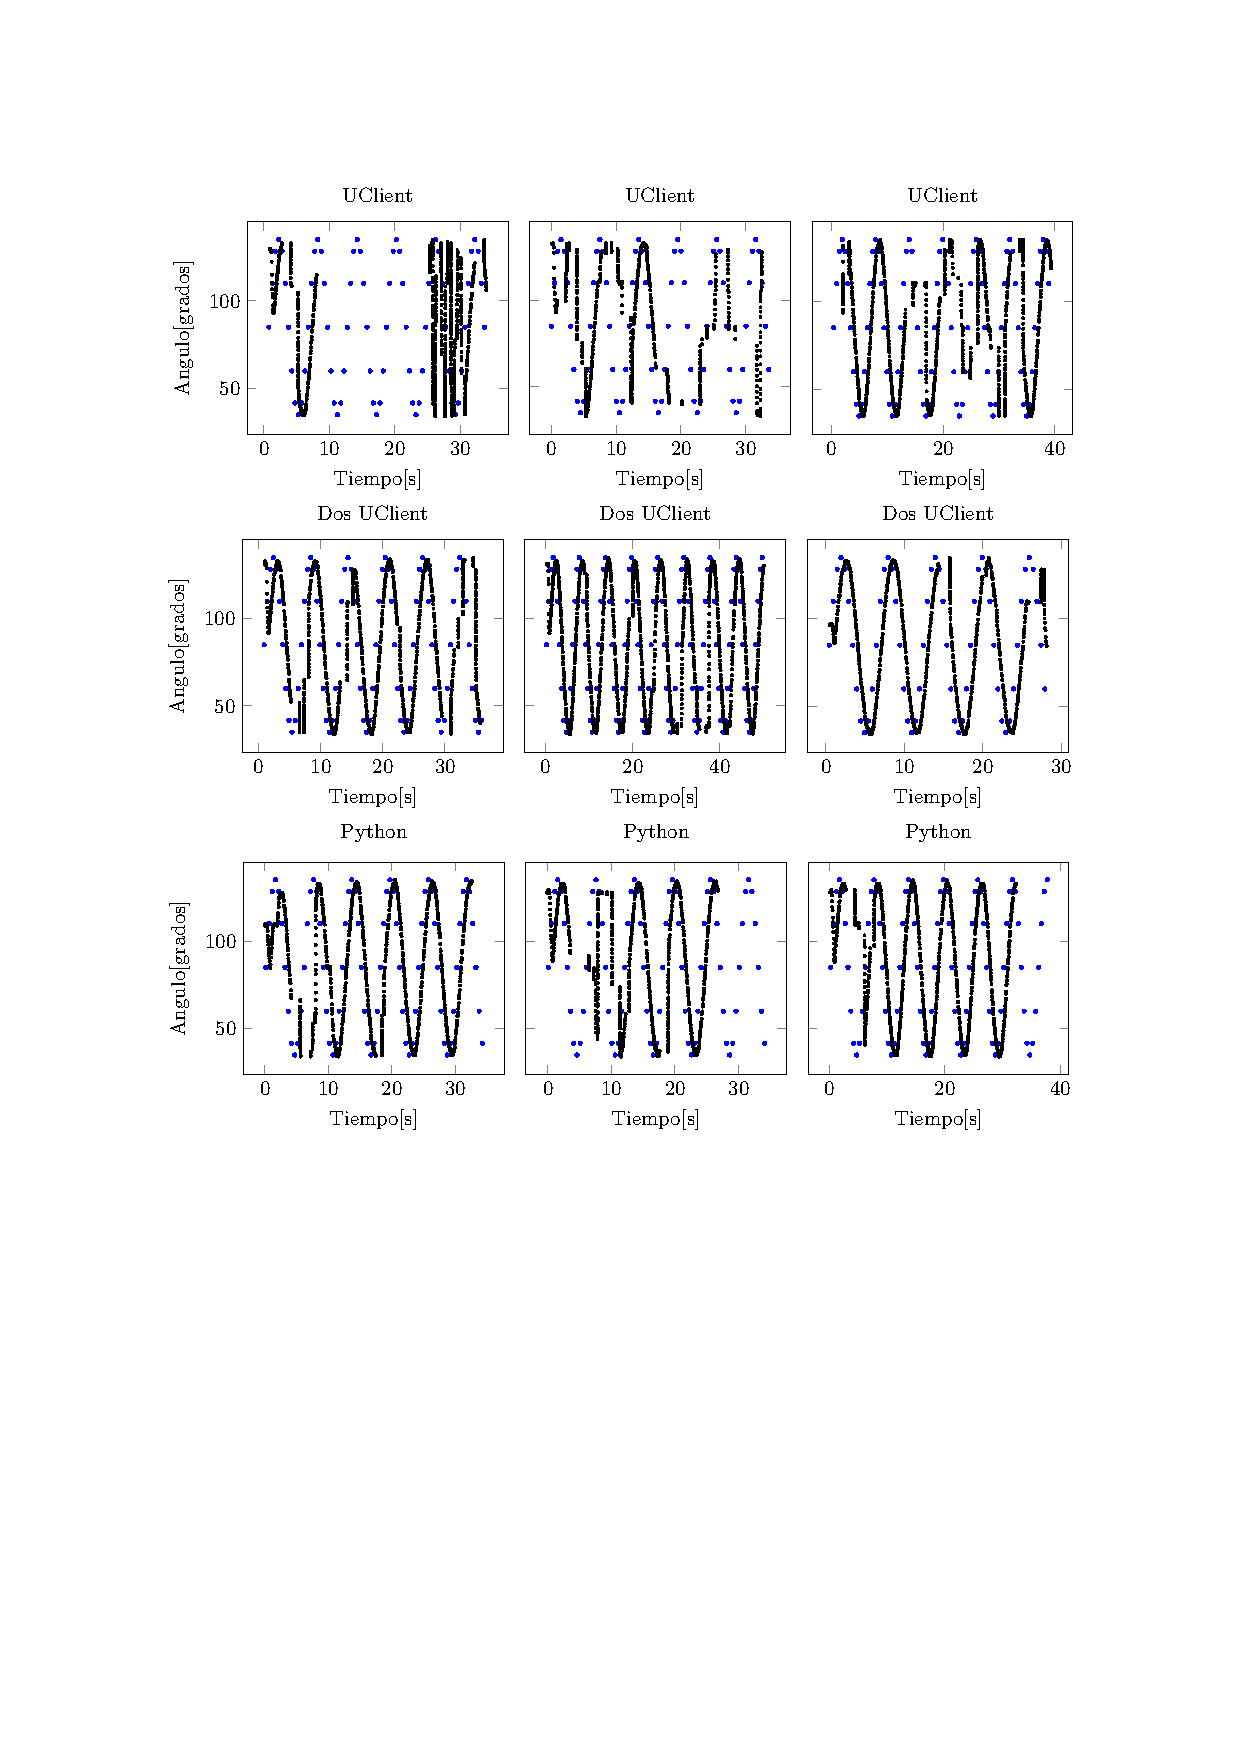
\includegraphics[scale=1]{plots/h2.pdf}
	 \caption{En azul, las posiciones enviadas a 2Hz y en negro las lecturas.}
  \label{fig:sin2H}
\end{figure}
\begin{figure}[H]
	\centering
   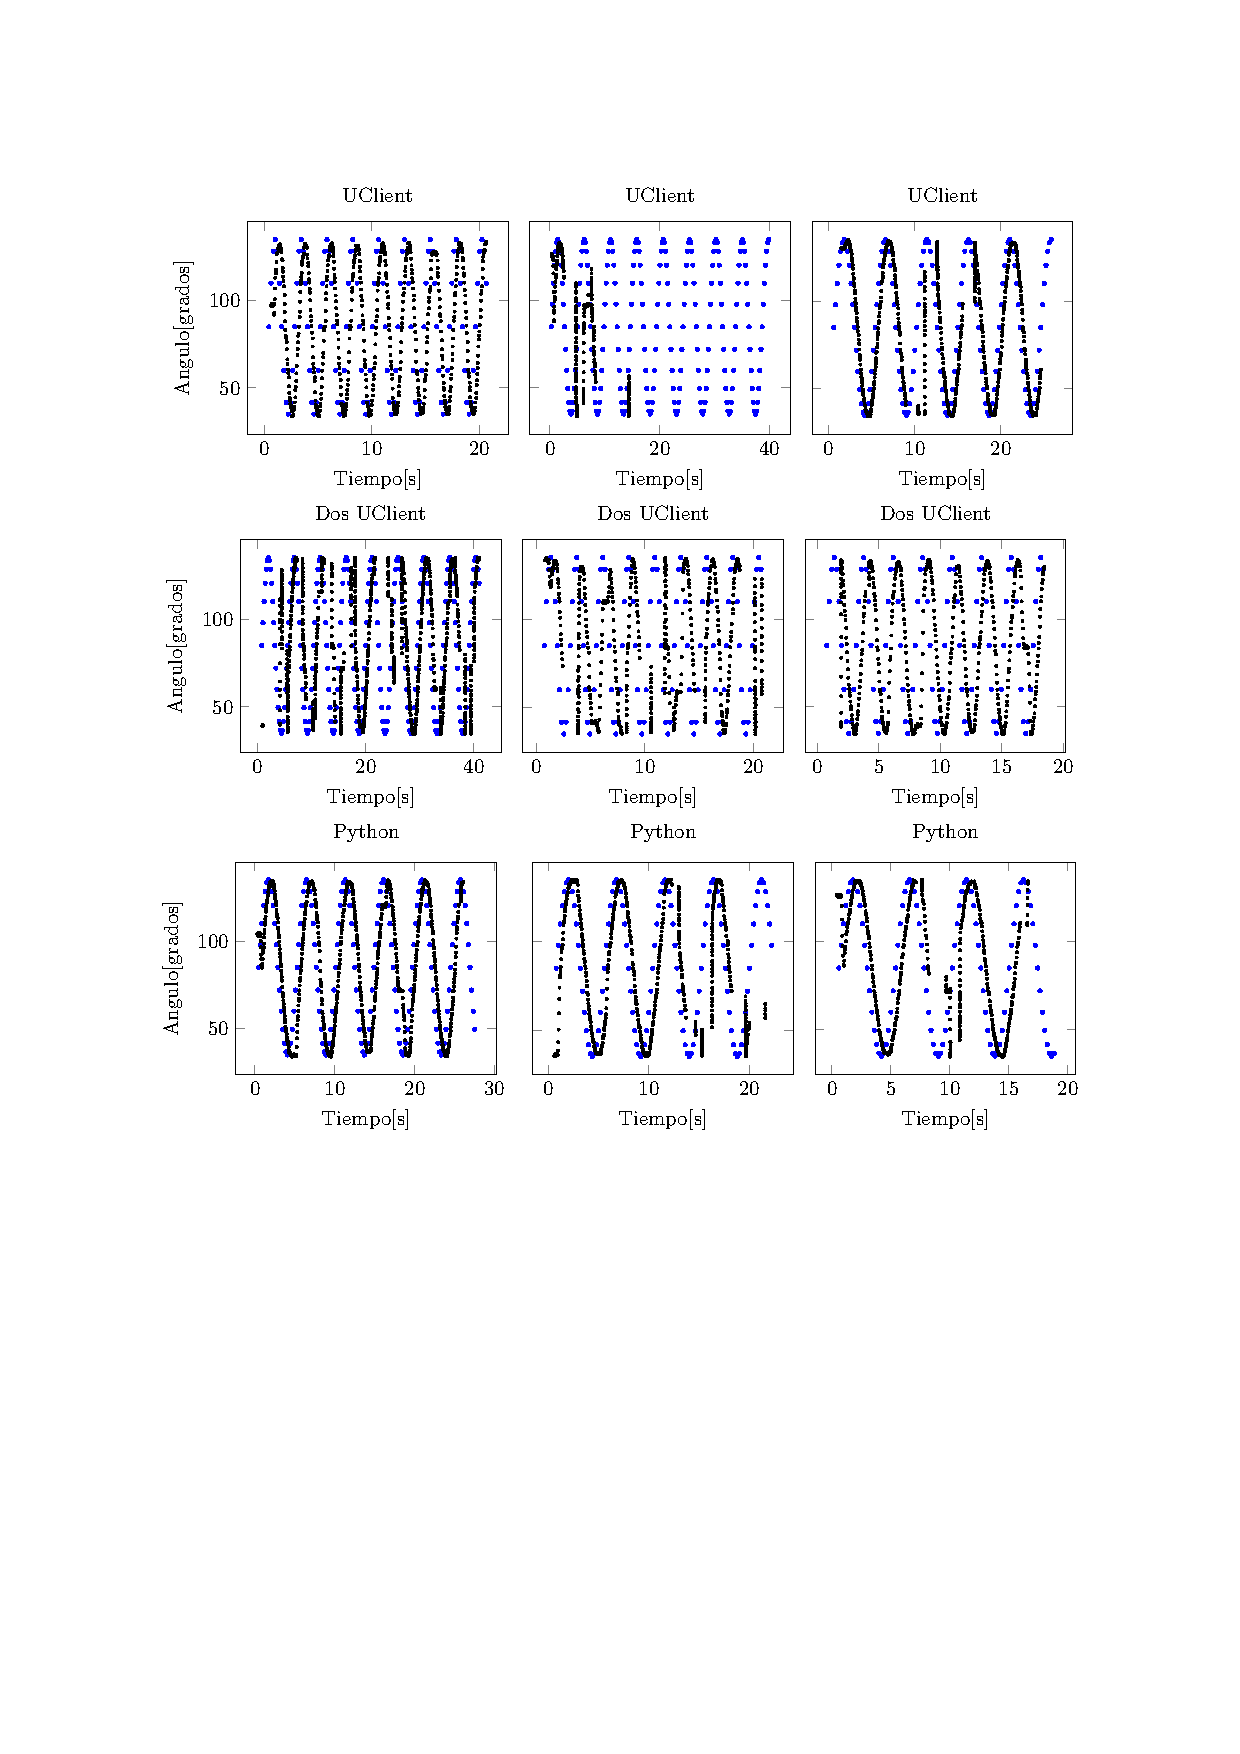
\includegraphics[scale=1]{plots/h5.pdf}
	 \caption{En azul, las posiciones enviadas a 5Hz y en negro las lecturas. }
  \label{fig:sin5H}
\end{figure}
\begin{figure}[H]
	\centering
    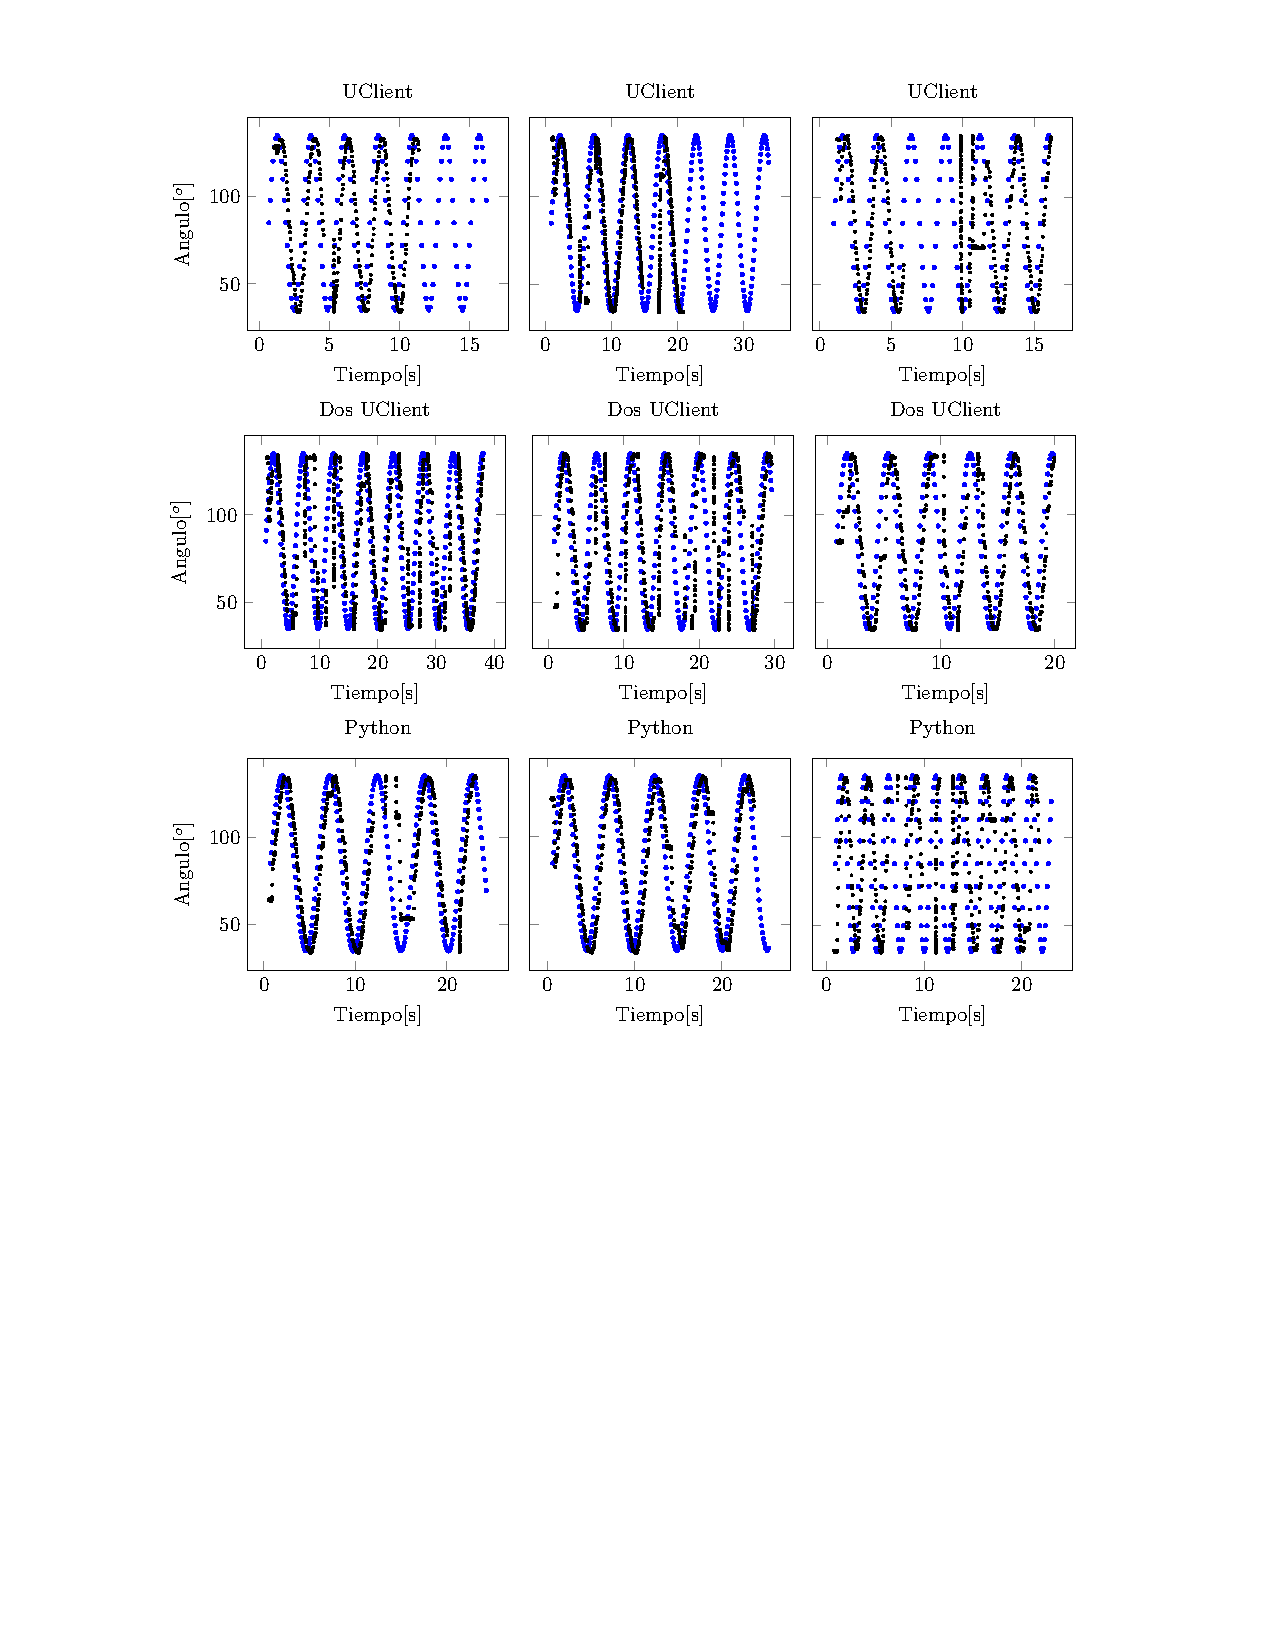
\includegraphics[scale=1]{plots/h10.pdf}
	 \caption{En azul, las posiciones enviadas a 10Hz y en negro las lecturas. }
  \label{fig:sin10H}
\end{figure}

En los gráficos anteriores se pueden distinguir dos tipos de errores que provocan que la trayectoria no sea la correcta:

\begin{itemize}
\item La articulación no se mueve: Reflejado como una recta negra horizontal y el modulo responsable es el de escritura.
\item No se recibe la posición actual: Reflejado como un periodo sin datos. En este caso no se puede saber si la articulación se ha movido\footnote{Por inspección visual se ha comprobado que ambos errores son independientes.}.
\end{itemize}
Se puede concluir que el seguimiento de la trayectoria es independiente de la frecuencia utilizada en este rango.
Por otro lado también se observa que con un solo cliente liburbi se producen grandes bloqueos en la recepción y muestra una trayectoria más discontinua e inconstante.
En los que respecta a los otros dos métodos, dos clientes con liburbi y python, tienen un comportamiento aceptable y no se puede no se puede concluir que uno sea mejor que otro. 

Para discernir cual de los dos métodos es más eficiente se han analizado las diferencias de tiempo entre el momento en que se envía la orden de los picos de la sinusoide y el momento en que se recibe que ha llegado a dicha posición. Para comprobar si existe diferencia entre las series se realiza una ANOVA sobre los datos de la Figura \ref{fig:retras}. Con un intervalo de confianza del 95\% el p-valor es de 2,1e-7, por lo tanto no se acepta la hipótesis nula y se puede concluir que el retraso con C++ es significativamente menor. 
 
\begin{figure}[H]
	\centering
\begin{tikzpicture}[baseline]
\pgfplotsset{width=10.5cm,compat=1.10}
\begin{axis}[
xlabel={réplicas},
ylabel={$tiempo[s]$},
minor y tick num=1,
%legend style={at={(0.5,-0.25)},
%anchor=north,legend columns=-1},
]
\addplot[blue, only marks] table {data/retrasoPy.dat};
\addplot[black, only marks] table {data/retrasoC++.dat};
\addplot[black,sharp plot,update limits=false]
coordinates {(0,0.399) (52,0.399)};
%node[above] at (axis cs:9,0.399) {0.399};
\addplot[blue,sharp plot,update limits=false]
coordinates {(0,0.733) (52,0.733)};
%node[above] at (axis cs:9,0.733) {0.733};
\legend{python, liburbi}
\end{axis}
\end{tikzpicture}

	 \caption{Retrasos entre la orden enviada y la acción.}
  \label{fig:retras}
\end{figure}

\section{Elección del método}

La elección del método que garantizará un mejor funcionamiento del paquete a implementar se realiza conforme a los criterios de evaluación resumidos en la Tabla \ref{comp}

\begin{table}[H]
\begin{center}
\begin{tabulary}{\textwidth}{|p{4cm}|p{3cm}|p{3cm}|p{3cm}|}
\hline

&\textbf{Python con telnet} & \textbf{C++ con liburbi y 1 cliente} & \textbf{C++ con liburbi y 2 clientes} \\ \hline
Frecuencia máxima de lectura [Hz]& 24.966,09 & 102.300,09 & 102.300,09 \\ \hline
Frecuencia media de lectura [Hz]& 13.610,99& 2.999,50 & 2.999,50  \\ \hline
Congelaciones en la lectura & Si & Si &Si \\ \hline
Frecuencia de envío& = & = & = \\ \hline
Seguimiento de trayectorias & Bueno & Malo & Bueno \\ \hline
Efecto negativo del envío en la lectura& No & Si & No \\ \hline
Retraso de la respuesta & Mayor & Menor & \\ \hline
Bloqueos en el envío & Si & Si & Si \\ \hline
\end{tabulary}
\end{center}
\caption{Esumen de los criterios de elección.\label{comp}}
\end{table}


En síntesis, el método liburbi se ha demostrado más eficaz en lo relativo a la recepción de datos, muestra un comportamiento similar a python en el seguimiento de las trayectorias con el uso de dos clientes y además se obtiene un retraso de seguimiento menor que python estadísticamente significativo. Adicionalmente, se ha de tener en consideración que el paquete será más complejo que los programas utilizados en los experimentos y dado que C++ se ejecuta a mayor velocidad que python las diferencias de ejecución podrían llegar a ser criticas.
En consecuencia la librería liburbi usando dos clientes es el método elegido para implementar el paquete de ROS.


\newpage
\chapter{Implementación del paquete de ROS}
\thispagestyle{fancy}
\section{ROS}
\label{ros}
ROS es el acrónimo de Robot Operating System que lejos de ser un sistema operativo es más bien un marco de trabajo que proporciona unas herramientas y unas librerías para ayudar a desarrollar software para aplicaciones de robótica. Proporciona entre otras facilidades abstracciones de hardware, controladores para dispositivos, herramientas de visualización, comunicación por mensajes, administración de paquetes y todo ello bajo licencia de software libre.
La principal característica sobre ROS es su sistema de comunicación. A bajo nivel está basado en el paso de mensajes que pueden ser leídos por diversos procesos simultáneamente. Dichos mensajes se escriben sobre unos canales de comunicación llamados \textit{tópicos} a los que se puede acceder mediante métodos de publicación y suscripción. Sobre los tópicos se puede publicar o suscribir desde un terminal o bien cualquier objeto de ROS denominados \textit{nodos}. Todos los nodos que se pretendan tener comunicados entre sí deben estar creados sobre el mismo núcleo o \textit{roscore}.


Todos los programas que se ejecutan sobre ROS deben ser creados dentro de un paquete y todo paquete de ROS debe contener una serie de archivos necesarios para su compilación. Los archivos necesarios son los siguientes.
\begin{itemize}
\item manifest.xml: Incluye información sobre el nombre del paquete, el autor, tipo de licencia y paquetes externos necesarios.
\item CMakelists.txt: Indica el uso de librerías, el uso de mensajes propios del paquete y se declaran los ejecutables.
\item mainpage.dox: Contiene un resumen explicativo del paquete.
\item Archivos ejecutables: ROS permite usar su API con C++ y python.
\item Carpeta msg: Contiene los archivos *.msg donde se definen los mensajes propios del paquete.
\item Carpeta srv: Contiene los archivos *.srv donde se definen los servicios propios del paquete.
\item Carpeta launch: Contiene los archivos *.launch que permiten lanzar varios nodos de diferentes paquetes y tipos, con los parámetros convenientes.

\end{itemize}
\subsection{Paquete aibo{\_}server }
Se pretende implementar un paquete que se conecte al AIBO dentro de una red local. Una vez conectado debe recoger los datos enviados por el servidor URBI del AIBO y publicarlos sobre una serie de tópicos. De forma inversa debe tratar los valores de las articulaciones del tópico al que está suscrito y enviarlos al servidor con el fin de actuar sobre la plataforma.

\begin{figure}[H]
	\centering
    \includegraphics[scale=0.6]{images/aiboserverNodo.pdf}
	 \caption{Nodo aibo{\_}server.}
  \label{fig:aiboserv}
\end{figure}

Para la realización de este paquete de ROS se han tenido en cuenta las siguientes consideraciones:
\begin{itemize}
\item Incluir en el manifest.xml los paquetes de ROS necesarios para su implementación:
\begin{itemize}
\item roscpp: Para utilizar la API ROS para C++.
\item std{\_}msgs: Permite el uso de mensajes estándar.
\item sensor{\_}msgs: Permite el uso de mensajes especialmente destinados a ciertos tipos de sensores.
\end{itemize}
\item Implementar los archivos necesarios para el ejecutable:
\begin{itemize}
\item AiboNode.cpp: Archivo a partir del cual se crea el ejecutable del paquete. En él reside la estructura del programa.
\item AiboServer.cpp y AiboServer.h: Se define la clase aibo en la que se basa AiboNode.cpp.
\item AiboParams.h: Se definen las constantes.
\end{itemize} 
\item Definir los mensajes propios:
\begin{itemize}
\item Accel.msg: Mensaje destinado al acelerómetro.
\item Bumper.msg y BumperArray.msg: Mensaje destinado a los sensores de contacto de las patas.
\item IRArray.msg: Mensaje destinado a los tres infrarojos.
\item Jointes.msg: Mensaje destinado a las articulaciones.
\item Sound.msg: Mensaje destinado al envío de sonido.
\item TouchArray.msg: Mensaje destinado a los sensores de tacto de la espalda y la cabeza.
\end{itemize}
\item Modificar el CMakeList.txt para incluir los mensajes y los archivos C++ anteriores junto con la librería liburbi.
\end{itemize}

\subsection{Estructura del programa}
 Conforme a lo indicado en la sección anterior, Sección \ref{seccomp}, se procede a la implementación del paquete de ros usando liburbi y dos clientes, uno para la recepción  y otro para el envío.

La estructura del programa implementado se puede ver en la Figura \ref{fig:aiboserver}.
\begin{figure}[H]
	\centering
    \includegraphics[scale=0.35]{images/Aibo_Server.pdf}
	 \caption{Estructura básica del ejecutable aibo{\_}server.}
  \label{fig:aiboserver}
\end{figure}
Siguiendo el esquema en la Figura \ref{fig:aiboserver} se detallan los diferentes bloques.
\begin{itemize}
\item Inicializaciones: 
\begin{itemize}
\item Inicialización del nodo de ROS:
\begin{itemize}
\item Creación del nodo: Se le otorga un identificador al nodo, en este caso aibo{\_}server.
\item Definición de la frecuencia de ejecución del bucle de ROS.
\item Se inicializa el \textit{Subscriber} que permitirá llamar al callback de ROS.   
\end{itemize}

\item Inicialización de la instancia de la clase \textbf{aibo}:
\begin{itemize}
\item Inicialización de los clientes URBI de lectura y escritura.
\item Creación de los tópicos e inicialización de los \textit{publishers} que publicaran en tópicos.
\item Definición del Callback de URBI para cada sensor y articulación.
\item Demanda del envío de datos desde URBI.
\item Definición del método de tratamiento de ordenes que usará el servidor URBI.
\end{itemize}
\end{itemize}
\item Bucle de URBI:
\begin{itemize}
\item Se crea un hilo de ejecución en paralelo donde se lleva acabo el bucle de URBI.
\item Llamada a los callbacks de URBI: En los callbacks se guardan los valores obtenidos en las variables de clase correspondientes.

\end{itemize}
\item Bucle de ROS:
\begin{itemize}
\item Publicación de las variables de los sensores y articulaciones en los tópicos correspondientes.
\item Llamada al callback de ROS: Éste envía la orden al servidor URBI mediante el cliente de envío.
\end{itemize}
\end{itemize}
\subsection{Resultados del aibo{\_}server}

Por lo que respecta la adquisición de los valores de sensores y articulaciones se ha conseguido obtenerlos trabajando a una frecuencia de 10Hz. Con el objeto de verificar que el refresco de los tópicos es correcto se ha accedido a mostrar por el terminal todos ellos junto con su frecuencia de refresco Figura \ref{fig:getT}, y al mismo tiempo, en la Figura \ref{fig:addacc} se representa el valor de un sensor. El hecho de que el gráfico muestre un cierto ruido indica que el valor se esta refrescando correctamente, por el contrario si el valor de la gráfica es constante indica que no se está refrescando correctamente.

\begin{figure}[H]
	%\centering
    \includegraphics[scale=0.3]{images/getTopics.png}
	 \caption{Consulta de la frecuencia de publicación en los diferentes tópicos de aibo{\_}server.}
  \label{fig:getT}
\end{figure}

\begin{figure}[H]
	\centering
    \includegraphics[scale=0.28]{images/accel.jpg}
	 \caption{Valores de los acelerómetros usando la herramienta rqt{\_}plot.}
  \label{fig:addacc}
\end{figure}

Para realizar una valoración del envío de las posiciones necesita de un paquete de ROS que permita cuantificar los resultados.

El test aplicado es similar al realizado en las experimentaciones de la Sección \ref{seccomp}. Se trata de enviar punto a punto una trayectoria sinusoidal a las posiciones de una articulación.
Para la realización del test se ha implementado un sencillo programa\footnote{El código se puede encontrar en el Anexo \ref{sinlegROS}} que crea un nodo que publica sobre el tópico \textit{/aibo{\_}server/aibo/subjoints/jointRF1}.
La estructura entre los nodos se muestra en la Figura \ref{fig:ASSL}.
\begin{figure}[H]
	\centering
    \includegraphics[scale=0.35]{images/rosgraphASsin.pdf}
	 \caption{Estructura de ROS con los nodos aibo\_server y SinLeg.}
  \label{fig:ASSL}
\end{figure}

De los resultados obtenidos en la realización de varias réplicas a diversas frecuencias se deduce que el seguimiento de la trayectoria lleva un retraso mínimo entorno a los 0.5 segundos, dato que coincide con el retraso medio obtenido en las experimentaciones de la sección \ref{secenvdades}. Si bien, como se puede observar en las Figuras \ref{fig:ASsin2Hz}, \ref{fig:ASsin7Hz} y \ref{fig:ASsin10Hz} 
dicho retraso no es la norma general estando el retraso medio es mayor al obtenido en las experimentaciones.
\begin{figure}[H]
	\centering
	    \includegraphics[scale=0.28]{images/10Ry2S.jpg}
 	\caption{Entrada y respuesta del sistema ante una señal sinusoidal de enviando puntos a 2Hz.}
  \label{fig:ASsin2Hz}
\end{figure}
\begin{figure}[H]
	\centering
    \includegraphics[scale=0.28]{images/10Ry7S.jpg}
 	\caption{Entrada y respuesta del sistema ante una señal sinusoidal de enviando puntos a 7Hz.}
  \label{fig:ASsin7Hz}
\end{figure}
   \begin{figure}[H]
	\centering
    \includegraphics[scale=0.28]{images/10Ry10SAll.jpg}
 	\caption{Entrada y respuesta del sistema ante una señal sinusoidal de enviando puntos a 10Hz.}
  \label{fig:ASsin10Hz}
\end{figure}

Por otro lado el modulo implantado no ha mejorado los resultados obtenidos en la sección \ref{secenvdades} en lo relativo a los bloqueos. Por lo tanto, cabe concluir que el módulo no proporciona las condiciones necesarias para aquellas aplicaciones en las que se requiere una lectura y una respuesta rápida del sistema. 

\subsection{Mejoras del aibo{\_}server}
Los problemas encontrados, tras un proceso se pueden clasificar de la siguiente forma:
\begin{itemize}
\item Cortas congelaciones en la recepción de los valores de los sensores y articulaciones: Ya se ha probado que en las experimentaciones anteriores que los resultados no podían mejorar usando liburbi.
\item Envío de la orden correcto pero el movimiento se realiza con una demora: Esto es debido a un problema interno en el tratamiento de las órdenes del servidor URBI y por lo tanto des del punto de vista del cliente no se puede aportar ninguna solución.
\item Bloqueos en el envío de la orden de movimiento: Dichos bloqueos se originan en la función de liburbi que envía ordenes provocando un bloqueo completo del nodo.
\end{itemize}

Aunque para los dos primeros problemas no existe una solución si se ha encontrado una solución para el bloqueo en el envío de las ordenes de movimiento. 
En primer lugar, cuando se produce un bloqueo en el envío, éste no debe afectar a la recepción de las demás variables. Como solución se propone que el envió y la recepción se produzcan en dos threads distintos e independientes. 
En segundo lugar, se desea evitar los bloqueos en el envío. Para ello se inicializa un tercer cliente URBI que remplace al cliente de envío en caso de que éste se bloquee. Igualmente en caso de bloqueo del nuevo cliente se espera que el primero, que ya se habrá reinicializado, tome el relevo.
Bajo estas ideas se ha reescrito el callback de ROS como muestra el diagrama de la figura \ref{fig:Call}.
\newpage
\begin{figure}[H]
	\centering
    \includegraphics[scale=0.7]{images/esquemaCall.pdf}
	 \caption{Diagrama del callback de ROS. Los flags \textit{anterior}, \textit{C1activo} y \textit{C2activo}  se inicializan con valor 1 y los flags \textit{reiniciando1} y \textit{reiniciando2} se inicializan a 0.}
  \label{fig:Call}
\end{figure}

Con esta modificación se ha conseguido que el envío de datos, que de forma natural con liburbi es síncrona, ya que la función de envío espera una respuesta del servidor, se trate de forma asíncrona. Este modo gana en velocidad de transmisión y evita los bloqueos pero no garantiza la llegada de todos los paquetes de datos.

Con la modificación introducida se vuelve a aplicar el test.
En la Figura \ref{fig:ASempiezamala} se ve como tras un primer seguimiento aceptable de la trayectoria empieza una zona donde el seguimiento empeora. Durante este periodo de tiempo que continua en la Figura \ref{fig:ASpeor} la comunicación con el AIBO es realmente mala y donde se originaran los bloqueos. Tras implementar el nuevo callback la comunicación no se corta, pero la trayectoria no se sigue correctamente.

\begin{figure}[H]
	\centering
    \includegraphics[scale=0.26]{images/empiezamala.jpg}
 	\caption{Empiezan a producirse bloqueos.}
  \label{fig:ASempiezamala}
\end{figure}
\begin{figure}[H]
	\centering
    \includegraphics[scale=0.26]{images/peora5hz.jpg}
 	\caption{Se producen bloqueos que se intentan evitar.}
  \label{fig:ASpeor}
\end{figure}

En la Figura \ref{fig:ASrecupera} se ve como , tras una serie de sucesivos bloqueos de ambos clientes, se eecupera un buen seguimiento de la trayectoria.
 
\begin{figure}[H]
	\centering
    \includegraphics[scale=0.26]{images/recupera.jpg}
 	\caption{Recuperación del seguimiento de la trayectoria.}
  \label{fig:ASrecupera}
\end{figure}

Finalmente en la Figura \ref{fig:ASbuena} se puede observar como en algunos momentos el seguimiento de la trayectoria es satisfactorio. 

Cabe señalar que en los gráficos obtenidos mediante la herramienta de ROS rqt{\_}plot no permiten diferenciar entre un error recepción de datos o un seguimiento de la trayectoria incorrecto. 
 \begin{figure}[H]
	\centering
    \includegraphics[scale=0.26]{images/mejor5hz.jpg}
 	\caption{Buen seguimiento de la trayectoria.}
  \label{fig:ASbuena}
\end{figure}



\section{Paquete Aibo{\_}description }
Este paquete pretende ser el vínculo entre el AIBO y una de las herramientas más usadas de ROS para robots móviles: rviz\footnote{http://wiki.ros.org/rviz}, un visualizador 3D para aplicaciones de robótica que permite visualizar un modelo, el entorno sensado o un mapa virtual. 

El paquete consta de dos partes diferenciadas, la creación del modelo de AIBO para su representación en imagen 3D y la implementación de un nodo que sincronice el modelo con el robot.

\subsection{El modelo}
Para generar un modelo, se debe editar un xml con formato URDF\footnote{http://wiki.ros.org/urdf}(Unified Robots Description Format) donde se especifican las dimensiones del robot, las articulaciones y sus movimientos, la geometría de las extremidades y parámetros físicos como la masa o la inercia.
Para el modelo del AIBO se han creado 22 partes y 21 articulaciones. Se han descartado en el modelo la boca y las orejas. En la Figura \ref{fig:aibourdf} Se puede ver un esquema de las articulaciones, las partes y la disposición de los ejes que conforman el modelo implementado en el archivo URDF.

%\newpage
\begin{figure}[H]
	\centering
    \includegraphics[scale=0.39]{images/Aibo.pdf}
	 \caption{Estructura del modelo URDF.}
  \label{fig:aibourdf}
\end{figure}

En  cada una de las partes se debe definir la geometría y sus dimensiones. Con el fin de darle un aspecto visual más atractivo y mas semejante más al AIBO real la geometría ha sido  definida mediante archivos .stl que contienen las figuras de cada una de las partes. A partir de un modelo solido se han dividido y modificado algunas piezas usando las softwares de apoyo FreeCAD\footnote{http://freecadweb.org/} y Netfabb\footnote{http://www.netfabb.com/}. El resultado desde la ventana de rviz se muestra en la Figura \ref{fig:aiborviz}.
 
\begin{figure}[H]
	\centering
    \includegraphics[scale=0.32]{images/aiborviz.png}
	 \caption{Modelo visto des de el framework de rviz.}
  \label{fig:aiborviz}
\end{figure}
\subsection{El nodo state{\_}publisher}\label{nodoSP}
El nodo state{\_}publisher esta creado mediante un programa escrito en C++ (state{\_}publisher.cpp) y está suscrito al tópico \texttt{/aibo{\_}server/ aibo/joints}, donde se encuentran las posiciones de las articulaciones del robot real, y las publica en un tópico llamado \texttt{joint{\_}states} al que accede rviz. Además envía la transformada del modelo cinemático.
La estructura del programa es la siguiente:
\begin{itemize}
\item Inicialización:
\begin{itemize}
\item Inicialización del nodo state{\_}publisher.
\item Inicialización del \textit{publisher}.
\item Inicialización del \textit{subscriber}.
\item Inicialización del \textit{broadcaster}: Canal de envió de la transformada. 
\end{itemize}
\item Declaración de mensajes:
\begin{itemize}
\item joint{\_}state:Donde se publica el estado de las articulaciones.
\item odom{\_}trans: Donde se envía la transformada.
\end{itemize}
\item Bucle de ROS:
\begin{itemize}
\item Actualización del estado de las articulaciones.
\item Actualización de la transformada.
\item Envío de las articulaciones.
\item Envío de la transformada.
\item Revisión del callback. 
\end{itemize}
\item Callback del \textit{subscriber}:
\begin{itemize}
\item Adquisición de los valores de las articulaciones.
\end{itemize}
\end{itemize}
\subsection{Estructura de paquete}
Para la realización del paquete se han implementado o modificado los siguientes archivos:
\begin{itemize}
\item Incluir en el manifest.xml los paquetes de ROS necesarios:
\begin{itemize}
\item roscpp: Permite usar el API de ROS para C++.
\item urdf: Permite leer y parsear archivos urdf.
\item std{\_}msg: Permite importar mensajes estándar.
\item tf: Permite la crear el modelo cinemático inverso.
\item aibo{\_}server: Permite importar los mensajes propios.  
\end{itemize}
\item Implementación del archivo state{\_}publisher.cpp, Sección \ref{nodoSP}.
\item Carpeta urdf: Se incluye el archivo Aibo.urdf donde está descrito el modelo.
\item Carpeta meshes: Se incluyen los archivo stl con los modelos 3D de las partes del modelo.
\item Carpeta launch: Incluye el archivo aibomod.launch. En el se definen los nodos y los parámetros a partir de los que será posible la visualización del modelo con rviz.
\begin{itemize}
\item Se asigna al parámetro robot{\_}description el archivo Aibo.urdf.
\item Se lanza un nodo del tipo robot{\_}state{\_}publisher del paquete con el mismo nombre. Dicho nodo está suscrito al tópico joint{\_}states sobre el que publica el nodo implementado, state{\_}publisher, y se encarga de leer el URDF del modelo que haya bajo el parámetro robot{\_}state{\_}publisher y publica sobre el tópico /tf el cual usa rviz para generar el movimiento del modelo.
\item Se lanza un nodo del tipo state{\_}publisher.
\item Se lanza un nodo del tipo rviz con la configuración deseada.
\end{itemize}
\end{itemize}

En la Figura \ref{fig:aibostack} se puede observar cómo queda la estructura de los nodos con el visualizador rviz y el nodo aibo{\_}server en funcionamiento.

\begin{figure}[H]
	\centering
    \includegraphics[scale=0.26]{images/graphModel.pdf}
	 \caption{Estructuras de los nodos de ROS con aibo{\_}server y el modelo visualizado con rviz.}
  \label{fig:aibostack}
\end{figure}
\newpage

\chapter{Presupuesto}
\thispagestyle{fancy}
El coste total del proyecto asciende a 18.200{\euro} de los cuales el 82,42{\%}corresponden a gastos de personal. Los costes asociados al material solo vienen dados por el coste de la plataforma de estudio. Ya que en ser un proyecto fundamentalmente de software y todo el software usado es con licencia libre, des de el sistema operativo hasta el procesador de textos, 

\section{Coste material}

\begin{table}[H]
\begin{center}
\begin{tabulary}{\textwidth}{|C|C|C|C|}
\hline
\textbf{Concepto}&\textbf{Coste unitario [{\euro}/unid.]} & \textbf{Cantidad} & \textbf{Coste total [\euro]} \\ \hline
AIBO ERS-7 & 1.600& 2& 3.200 \\ \hline

\end{tabulary}
\end{center}
\caption{Coste material detallado.\label{costmat}}
\end{table}
\section{Coste personal}
\begin{table}[H]
\begin{center}
\begin{tabulary}{\textwidth}{|C|C|C|C|}
\hline
\textbf{Concepto}&\textbf{Coste horario [{\euro}/hora]} & \textbf{Horas} & \textbf{Coste total [\euro]} \\ \hline
Estudio preliminar & 30& 300& 9.000 \\ \hline
Diseño y depuración & 30& 150& 4.500 \\ \hline
Programación& 15& 100& 1.500 \\ \hline
\textbf{Total}& & 550& 15.000 \\ \hline
\end{tabulary}
\end{center}
\caption{Coste personal detallado.\label{costper}}
\end{table}

\newpage

\chapter{Impacto ambiental}
\thispagestyle{fancy}
El objetivo de este proyecto conlleva como causa inmediata el incremento de la vida útil de una plataforma ya en desuso. Y en este sentido cabe entenderlo como el reciclaje de un objeto que de otro modo acabaría por desecharse en poco tiempo.

El ahorro en los costes ambientales asociados al uso de la plataforma se puede dividir en chasis, electrónica y batería.

El chasis esta hecho de ABS (Acrilonitrilo Butadieno Estireno, en inglés). Se trata de un termoplástico amorfo difícil de reciclar y en su proceso de fabricación usa acrilonitrilo, que es altamente tóxico.

Tanto la electrónica como las baterías contienen metales pesados altamente contaminantes si no son tratados correctamente.

Las baterías son de iones de litio y aunque su impacto ambiental no está del todo claro, tienen potencial de contaminar el subministro de agua subterránea debido a que contiene metales como cobalto.


\newpage
\chapter*{Conclusiones}
\thispagestyle{fancy}
\addcontentsline{toc}{chapter}{Conclusiones}
Se ha alcanzado el objetivo implementando los paquetes \textbf{aibo{\_}server} y \textbf{aibo{\_}description}. Estos paquetes están disponibles para su uso o modificación con tal de complementarlos o mejorar los resultados (\url{https://github.com/Diamg/AiboRosPackages}). 
El módulo implementado permite adquirir los datos de los sensores y articulaciones del AIBO de forma satisfactoria a velocidades superiores a 10 Hz en forma de tópicos de ROS. Esta parte del módulo por si solo ya facilita enormemente la programación y sobretodo el testeo y la depuración con el uso de las herramientas que facilita ROS. Además en esta linea se ha incluido un modelo para el visualizador rviz con un aspecto visual y funcional complementando el módulo anterior.  
Por otro lado la parte implementada que se encarga de enviar las ordenes al AIBO permitiendo actuar sobre el no se ha dado muy buenos resultados y no permite el envío de trayectorias punto a punto con este método. De todos modos URBI tiene su propio generador de trayectorias por lo que permite enviar funciones de movimiento más complejas  o posiciones concretas enviadas a un ritmo mas bajo del implementado.

Este proyecto deja un camino abierto a las posibles mejoras y complementos. Entre otros la integración del modulo de visión y audio usando URBI como se ha echo. Por otra parte cabe la duda de si el comportamiento de envío sería mejor usando OPEN-R, al eliminar una capa de programación intermedia, URBI, que posiblemente ralentice y empeore la comunicación entre cliente y servidor. En cuanto al modelo y el nodo que permite su integración con rviz podría completarse añadiendo los sensores del AIBO como los acelerómetros, los infrarrojos, los sensores de presión y contacto y la camera, permitiendo entre otros proyectos de odometría.

A nivel personal y educativo este proyecto ha servido para poner a prueba la capacidad de análisis y de resolución de problemas. Ha ayudado a tener un amplio conocimiento de de uno de los frameworks relacionados con la robótica mas usados del momento. Además a ayudado a mejorar las habilidades de desarrollo de software con los lenguajes C++ y python. 

\newpage
\chapter*{Agradecimientos}
\thispagestyle{fancy}
\addcontentsline{toc}{chapter}{Agradecimientos}
Este proyecto no podría haber sido posible sin el apoyo de la familia y amigos que han sido fuente de motivación y ánimo.

Un especial agradecimiento a los tutores de éste proyecto, Manel Velasco y Cecilio Angulo tanto por su implicación y atención como por facilitar el material y el espacio de trabajo.

Por último agradecer al doctor Ricardo Tellez de quien salió la idea de este proyecto y quien le dio su primer impulso, además de su apoyo y consejo durante su realización.
\newpage
\clearpage
\addcontentsline{toc}{chapter}{Referencias}
\thispagestyle{fancy}
\begin{thebibliography}{99}

\bibitem{aibo}
	Arevalillo-Herráez, Miguel and Moreno-Picot, Salvador and Millán, Vicente Cavero,
	\emph{Arquitectura para Utilizar Robots AIBO en la Enseñanza de la Inteligencia Artificial.}
	2012.
	\url{http://dblp.uni-trier.de/db/journals/ieee-rita/ieee-rita6.html#Arevalillo-HerraezMM11},
	
\bibitem{ros}
	Quigley, Morgan and Conley, Ken and Gerkey, Brian P. and Faust, Josh and Foote, Tully and Leibs, Jeremy and Wheeler, Rob and Ng, Andrew Y.,
	\emph{ROS: an open-source Robot Operating System}.
	2009.
\bibitem{libroblanco}
	CEA, Comité Español de Automàtica,
	\emph{El libro blanco de la robótica en España}.
	2011.
	
\bibitem{OPEN-R PG}
  Sony Corporation,
  \emph{OPEN-R Programmer's Guide}.
  2004.

\bibitem{urbiref}
	Baillie,
	\emph{URBI: Towards a Universal Robotic Low-Level Programming Language}.
	2005.
	
\bibitem{xavi}
	Xavier Perez,
	\emph{Vision-based Navigation and Reinforcement Learning Path Finding for Social Robots}.
	2010.
\bibitem{metod}
	Ángel Montero Mora, Gustavo Méndez Muñoz, José Ramon Dominguez Rodriguez,
	\emph{Metodologías de diseño de comportamientos para AIBO ERS7}.
	2009.
\bibitem{robocup}
	RoboCup, \url{http://www.robocup2014.org/}
\bibitem{morales}
	Jesus Morales,
	\emph{Localización de objetos y posicionamiento en el escenario de RoboCup Four-Legged con un robot AIBO}.
	2007.  
\bibitem{jesus}
	Jesús Martinez Gómez, 
	\emph{Diseño de un teleoperador con detección de colisiones para robots AIBO}. 			2006.
\bibitem{riki}
	Ricardo A. Tellez,
	\emph{Aibo Programming}.
	\url{http://www.ouroboros.org/aibo.html}
\bibitem{TekkQuickRef}
	Ethan Tira-Thompson,
	\emph{Tekkotsu Quick Reference}, ERS-7, Tekkotsu 3.0.
\bibitem{tekkTut}
	David S. Touretzky and Ethan J. Tira-Thompson, 
	\emph{Exploring Tekkotsu Programming on Mobile Robots}.
	Carnegie Mellon University,
	2010.
	\url{http://www.cs.cmu.edu/~dst/Tekkotsu/Tutorial/contents.shtml}
\bibitem{urbi}
	\emph{URBI},
	\url{http://www.urbiforge.org/index.php/Main/Robots}
	
\bibitem{urbicmd}
	Jean-Christophe Baillie,
	\emph{URBI Doc for Aibo ERS2xx ERS7 Devices documentation}.
	2005.

\bibitem{euslisp}
	ROS new by kwc,
	\emph{EusLisp now open source}.
	2010.
	\url{http://www.ros.org/news/2010/07/euslisp-now-open-source.html}
\bibitem{kecsap}
	Kecsap,
	\emph{Porting URBI 2.x for AIBO}.
	2010.
	\url{http://kecsapblog.blogspot.com.es/2010/12/porting-urbi-2x-for-aibo.html}
	
	
\end{thebibliography}

\label{Referencies}
%\addcontentsline{toc}{section}{Referències}
%\bibliography{Aibobib.bib}

\appendix
\clearpage % o \cleardoublepage
\addappheadtotoc
%\appendixpage

\chapter{Manual de usuario}\label{MU}
\thispagestyle{fancy}
\section{Requisitos previos}
Es necesario antes de instalar los paquetes seguir los siguientes pasos.

\begin{itemize}
\item Instalar Ubuntu 12.04 (Precise) de 32 bits.

\url{http://releases.ubuntu.com/12.04/}

\item Descargar librería liburbi 1.5 para C++:

\url{http://www.gostai.com/downloads/urbi/1.5/}
\begin{itemize}
\item Descomprimir la librería, que ya está compilada, en el directorio \texttt{/usr} del sistema.
\end{itemize}
\item Instalar de ROS. 

\begin{itemize}
\item Preparar el ordenador apara aceptar el software de ROS:


\begin{lstlisting}[language=bash]
  sudo sh -c 'echo "deb http://packages.ros.org/ros/ubuntu precise main" > /etc/apt/sources.list.d/ros-latest.list'
\end{lstlisting}

\item Preparación las claves:
\begin{lstlisting}[language=bash]
	wget http://packages.ros.org/ros.key -O - | sudo apt-key add -
\end{lstlisting}

\item Instalación:
\begin{lstlisting}[language=bash]
	sudo apt-get install ros-fuerte-desktop-full
\end{lstlisting}

\item Preparación del entorno:
\begin{lstlisting}[language=bash]
	echo "source /opt/ros/fuerte/setup.bash" >> ~/.bashrc
. ~/.bashrc
\end{lstlisting}

\item Crear un workspace:
\begin{lstlisting}[language=bash]
	rosws init ~/fuerte_workspace /opt/ros/fuerte
\end{lstlisting}
\begin{lstlisting}[language=bash]
	sudo apt-get install python-rosinstall
\end{lstlisting}
\item Crear un sandbox donde irán los nuevos paquetes y añadir al ROS{\_}PACKAGE{\_}PATH:
\begin{lstlisting}[language=bash]
	mkdir ~/fuerte_workspace/sandbox
	rosws set ~/fuerte_workspace/sandbox
	echo "source ~/fuerte_workspace/setup.bash" >> ~/.bashrc
. ~/.bashrc
	
\end{lstlisting}
\item Confirmación de la correcta instalación del entorno:

Al ejecutar:
\begin{lstlisting}[language=bash]
	echo $ROS_PACKAGE_PATH
\end{lstlisting}
Se debe obtener algo similar a:
\begin{lstlisting}[language=bash]
	/home/your_user_name/fuerte_workspace/sandbox:/opt/ros/fuerte/share:/opt/ros/fuerte/stacks
\end{lstlisting}
\end{itemize}

\item Asegurarse que los siguientes paquetes de ROS han sido instalados:
\begin{itemize}
\item rviz:
\begin{lstlisting}[language=bash]
	rospack find rviz
\end{lstlisting}
\item urdf
\begin{lstlisting}[language=bash]
	rospack find urdf
\end{lstlisting}
\item robot{\_}state{\_}publisher
\begin{lstlisting}[language=bash]
	rospack find robot_state_publisher
\end{lstlisting}
\item tf
\begin{lstlisting}[language=bash]
	rospack find tf
\end{lstlisting}


Deben devolver la ubicación del paquete.
\end{itemize}

\item Descargar los paquetes:
\begin{itemize}
\item aibo{\_}server:

\url{https://github.com/Diamg/AiboRosPackages/tree/master/aibo_server}
\item aibo{\_}description

\url{https://github.com/Diamg/AiboRosPackages/tree/master/aibo_description}
\end{itemize}
\item Copiar la tarjeta de memoria, Figura \ref{fig:aiboMS} para el AIBO con URBI:

\url{https://github.com/Diamg/AiboRosPackages/tree/master/MS_URBI}
\begin{figure}[H]
	\centering
    \includegraphics[scale=0.5]{images/MS.jpg}
	 \caption{Tarjeta de memoria para AIBO.}
  \label{fig:aiboMS}
\end{figure}

\item Configuración de la conexión wireless con el AIBO.

Editar el archivo WLANDFLT.txt que se encuentra en el directorio /OPEN-R/SYSTEM/CONF de la tarjeta de memoria del AIBO.

El archivo contiene los siguientes variables:
\begin{itemize}
\item HOSTNAME: Especifica el nombre de AIBO que se está usando.
\item ETHER{\_}IP: La IP que usará el AIBO.
\item ETHER{\_}NETMASK: La mascara de subred.
\item IP{\_}GATEWAY: La IP a traves de la que el AIBO accederá a la red.
\item ESSID: Nombre de la red inalámbrica.
\item WEPENABLE: con valor 1 si existe contraseña en la red o 0 en caso contrario.
\item WEPKEY: contraseña de la red.
\item APMODE: Método de conexión del AIBO.
\begin{itemize}
\item 0 para conexión punto a punto.
\item 1 para conexión con ruter.
\item 2 para conexión automática en el método que primero se lo permita.
\end{itemize}
\item CHANEL: especificar el canal para el modo punto a punto.
\end{itemize}
La configuración por defecto es:

HOSTNAME = AIBO

ETHER{\_}IP = 10.0.1.100

ETHER{\_}NETMASK = 255.255.255.0

IP{\_}GATEWAY = 10.0.1.1

ESSID = AIBONET

WEPENABLE = 1

WEPKEY = AIBO2

APMODE = 2

CHANNEL = 3 
\end{itemize}

\section{Instalación}
\begin{itemize}
\item Guardar los paquetes en el workspace de ROS.
\item Ejecutar en un terminal:
\begin{lstlisting}[language=bash]
	rosmake --pre-clean aibo_server
	rosmake --pre-clean aibo_description
\end{lstlisting}


\end{itemize}
\section{aibo{\_}server}
Ejecutar en terminal:
\begin{lstlisting}[language=bash]
	rosrun aibo_server aibo_server arg[1] arg[2]
\end{lstlisting}



Donde:
\begin{itemize}
\item arg[1] es la IP del AIBO.
\item arg[2] es la frecuencia en numero entero a la que se desea que vaya el bucle de ROS (La frecuencia por defecto y recomendada son 5 Hz).
\end{itemize}


\subsection{Tópicos}

El nodo aibo{\_}server permite subscribirse a los siguientes tópicos:
\begin{itemize}
\item \texttt{/aibo{\_}server/aibo/infrared}:
 
Da la información de los tres infrarojos del AIBO guardada en forma de mensaje de tipo aibo{\_}server/IRArrays.  

\item \texttt{/aibo{\_}server/aibo/touch}:

D la información de los sensores de presión de la barbilla, la cabeza y los tres de la espalda en un mensaje de tipo aibo{\_}server/TouchArray.

\item \texttt{/aibo{\_}server/aibo/accel}:

Da la información de los acelerometros en un mensaje de tipo aibo{\_}server/Accel.

\item \texttt{/aibo{\_}server/aibo/joints}:

Da la información de las posiciones de las articulaciones en un mensaje de tipo aibo{\_}server/Joints.

\item \texttt{/aibo{\_}server/aibo/paws}:

Da la información de los sensores de contacto de las tres patas en forma de mensaje del tipo aibo{\_}server/BumperArray.


\end{itemize}
Y publicar sobre el tópico:
\begin{itemize}
\item \texttt{/aibo{\_}server/aibo/subJoints}:

Permite controlar la posición de las articulaciones en un mensaje de tipo aibo{\_}server/Joints.

\end{itemize}

\subsection{Mensajes}
\begin{itemize}
\item aibo{\_}server/IRArrays

\begin{lstlisting}[language=bash]
	Header header
	sensor_msgs/Range[] IRs
\end{lstlisting}

El array de mensajes de tipo std{\_}msgs/Range esta ordenado:

\begin{table}[H]
\begin{center}
\begin{tabulary}{\textwidth}{|C|C|C|C|}
\hline
\textbf{Sensor}&\textbf{Máximo} & \textbf{Mínimo} & \textbf{Unidades} \\ \hline
Pecho & 90& 19& [cm] \\ \hline
Morro de corto alcance & 50& 5.7& [cm] \\ \hline
Morro de largo alcance & 20& 150& [cm] \\ \hline

\end{tabulary}
\end{center}
\end{table}
\item sensor{\_}msgs/Range
\begin{lstlisting}[language=bash]
	Header header         
	uint8 ULTRASOUND=0
	uint8 INFRARED=1
	uint8 radiation_type             
	float32 field_of_view  
	float32 min_range      
	float32 max_range      
	min_range==max_range
	float32 range           
                       
\end{lstlisting}
Se trata de un mensaje estándar de ROS\footnote{\url{http://docs.ros.org/api/sensor_msgs/html/msg/Range.html}}
\item aibo{\_}server/TouchArray

\begin{lstlisting}[language=bash]
	Header header
	float64[] touch
\end{lstlisting}


Los sensores están ordenados en la array de la siguiente forma:


\begin{table}[H]
\begin{center}
\begin{tabulary}{\textwidth}{|C|C|C|C|}
\hline
\textbf{Sensor}&\textbf{Máximo} & \textbf{Mínimo} & \textbf{Unidades} \\ \hline
Barbilla & 0& 1& [booleano] \\ \hline
Espalda delantero & 60& 0& [$\mu$Pa] \\ \hline
Espalda del medio & 60&0& [$\mu$Pa] \\ \hline
Espalda trasero & 60& 0& [$\mu$Pa] \\ \hline
Cabeza & 35& 0& [$\mu$Pa] \\ \hline
\end{tabulary}
\end{center}
\end{table}

\item aibo{\_}server/Accel:

\begin{lstlisting}[language=bash]
	Header header
	float64 x
	float64 y
	float64 z
\end{lstlisting}
\begin{itemize}
\item x: Valor del acelerometro en el eje x.
\item y: Valor del acelerometro en el eje y.
\item z: Valor del acelerometro en el eje z.
\end{itemize}
\begin{table}[H]
\begin{center}
\begin{tabulary}{\textwidth}{|C|C|C|C|}
\hline
\textbf{Sensor}&\textbf{Máximo} & \textbf{Mínimo} & \textbf{Unidades} \\ \hline
 x: Valor del acelerometro en el eje x. & -19,613& 19,613& [$m/s^2$] \\ \hline
y: Valor del acelerometro en el eje y. & -19,613& 19,613& [$m/s^2$] \\ \hline
z: Valor del acelerometro en el eje z. & -19,613& 19,613& [$m/s^2$] \\ \hline

\end{tabulary}
\end{center}
\end{table}
\item aibo{\_}server/Joints
\begin{lstlisting}[language=bash]
	Header header
	float64 jointLF1
	float64 jointLF2     
	float64 jointLF3     
	float64 jointLH1     
	float64 jointLH2 
	float64 jointLH3 
	float64 jointRF1
	float64 jointRF2
	float64 jointRF3
	float64 jointRH1
	float64 jointRH2
	float64 jointRH3
	float64 tailPan
	float64 tailTilt
	float64 headTilt
	float64 headPan
	float64 headNeck
	float64 mouth

\end{lstlisting}

Donde:
\begin{itemize}
\item jointLF1: Articulación de rotación del hombro del de la pata izquierda delantera.
\item jointLF2: Articulación de apertura del hombro de la pata izquierda delantera.
\item jointLF3: Articulación del codo de la pata izquierda delantera.  
\item jointLH1: Articulación de rotación del hombro del de la pata izquierda trasera.     
\item jointLH2: Articulación de apertura del hombro de la pata izquierda trasera.
\item jointLH3: Articulación del codo de la pata izquierda delantera.
\item jointRF1: Articulación de rotación del hombro del de la pata derecha delantera.
\item jointRF2: Articulación de apertura del hombro de la pata derecha delantera.
\item jointRF3: Articulación del codo de la pata derecha delantera.
\item jointRH1: Articulación de rotación del hombro del de la pata derecha trasera.
\item jointRH2: Articulación de apertura del hombro de la pata derecha trasera.
\item jointRH3: Articulación del codo de la pata derecha trasera.
\item tailPan: Articulación de la cola para el movimiento lateral.
\item tailTilt: Articulación de la cola para el movimiento vertical.
\item headTilt: Articulación de la cabeza para el movimiento vertical.
\item headPan: Articulación de la cabeza para el movimiento lateral.
\item headNeck: Articulación del cuello.
\item mouth: articulación de la boca.

\end{itemize}
\begin{table}[H]
\begin{center}
\begin{tabulary}{\textwidth}{|C|C|C|C|}
\hline
\textbf{Sensor}&\textbf{Máximo} & \textbf{Mínimo} & \textbf{Unidades} \\ \hline
jointLF1 & 134&-120&  [º] \\ \hline
jointLF2 & 91& -9& [º] \\ \hline
jointLF3 & 119&  -29& [º] \\ \hline
jointLH1 & 134& -120&  [º] \\ \hline
jointLH2 & 91&-9&  [º] \\ \hline
jointLH3 & 119&-29& [º] \\ \hline
jointRF1 & 120& -134& [º] \\ \hline
jointRF2 & 91& -9& [º] \\ \hline
jointRF3 & 119& -29& [º] \\ \hline
jointRH1 & 120& -134& [º] \\ \hline
jointRH2 & 91& -9& [º] \\ \hline
jointRH3 & 119& -29& [º] \\ \hline
tailPan & 59& -59& [º] \\ \hline
tailTilt & 63&2& [º] \\ \hline
headTilt & 44& -16& [º] \\ \hline
headPan & 91& -91& [º] \\ \hline
headNeck & 2& -79& [º] \\ \hline
mouth & -3& -58& [º] \\ \hline
\end{tabulary}
\end{center}
\end{table}

\item aibo{\_}server/BumperArray
\begin{lstlisting}[language=bash]
	Header header
	float64[] paws
\end{lstlisting}

La array de paws esta ordenada con el siguiente orden:

\begin{table}[H]
\begin{center}
\begin{tabulary}{\textwidth}{|C|C|C|C|}
\hline
\textbf{Sensor}&\textbf{Máximo} & \textbf{Mínimo} & \textbf{Unidades} \\ \hline
Delantero izquierdo & 1&0&  [booleano] \\ \hline
Trasero izquierdo & 1&0&  [booleano] \\ \hline
Delantero derecho & 1&0&  [booleano] \\ \hline
Trasero derecho & 1&0&  [booleano] \\ \hline
\end{tabulary}
\end{center}
\end{table}
\end{itemize}

\section{aibo{\_}description}
Ejecutar en la terminal:
\begin{lstlisting}[language=bash]
	roslaunch aibo_description aibomod.launch
\end{lstlisting}


Con tal de vincular el modelo con un AIBO se debe lanzar también un nodo aibo{\_}server.

\newpage

\chapter{Scripts y programas}
\thispagestyle{fancy}
\section{Adquisición del valor de una articulación con liburbi.}
\label{getDataOneLegC++}
\lstinputlisting[language=c++]{src/getDataOneLeg/getDataC++/getData.cpp}

\section{Adquisición del valor de una articulación con Python.}
\label{getDataOneLegPy}
\lstinputlisting[language=Python]{src/getDataOneLeg/getDataPython/getData.py}

\section{Envió de trayectoria punto a punto con liburbi.}\label{sinC}
\lstinputlisting[language=c++]{src/sinLegRead/sinLegC++/2Client/sinLeg.cpp}

\section{Envió de trayectoria punto a punto con Python.}\label{sinP}
\lstinputlisting[language=Python]{src//sinLegRead/sinLegPython/sinlegLF1.py}

\section{Envió de trayectoria punto a punto con ROS.}\label{sinlegROS}
\lstinputlisting[language=c++]{src/ROStests/sinlegROS.cpp}

\section{Modulo de imitación entre AIBOs.}\label{mimiccode}
\lstinputlisting[language=c++]{src/ROStests/mimic.cpp}

\end{document}
